\section{Exploration of learning preconditioners}
Now that we have the necessary theory about the iterative solver and their convergence. The two first thing that need to be done in this exploration of learning a preconditioner, is to determine the structure of our preconditioner and the algorithm that will learn the preconditioner

% do the learning of a preconditioner. 
 


\subsection{Structure of the preconditioner}\label{sec: initial par shift}
The two main structure properties that the preconditioner must have is, first that is easy to apply to a vector. As mentioned in section \ref{sec: prelim precond} the extra matrix vector products that is need to be done in each of the solvers iterations, regardless of the specific solver used, but is more prevalent for the more complicated methods. The simplest way to ensure a lower computational cost of a matrix vector product is to use preconditioner which is sparse. It can therefore be implemented as a CSR Matrix, which has the computational cost of the matrix vector product proportional to the number of nonzero values in the matrix \cite{Bai2000}. Another benefit from limiting to strictly sparse preconditioning matrices is the storage requirement is decreased significantly.

The second is the degrees of freedom most be kept relatively low, as what we are trying to achieve is to learn a preconditioner that lowers the solver iteration count. The key point is to learn, as the number of degrees of freedom determines how may different preconditioning matrices that can be found. This is a balance between of how fast it can it can explore the space of matrices, which in theory equates to faster learning. With fewer degrees of freedom. Against slower learning but with the possibility of finding a better preconditioner. With a higher degree of freedom.

The structure we have chosen to achieve these properties is to use an identity diagonal and partition the 1st superdiagonal into \(m\) as equal sized parts as possible. Because the matrix shift each elements of a vector by the next elements times a coefficient, we will call this preconditioning a partitioned shift preconditioner. The sparsity of this type of matrix is clear, as it has 2 nonzero elements per row beside the last row with 1 nonzero element. With this construction it is easy to control the degrees of freedom for testing different sizes, as it is equal to the number of partitions \(m\).

\begin{equation}\label{eq: par shift precond}
    \begin{pmatrix}
    1 & x_1 & 0\\
    0 & 1 & x_1 & 0 \\
    &0& 1 & x_2 & 0 \\
    &&&\ddots & \ddots\\
    &&&0&1 & x_{m-1} & 0\\
    &&&&0&1 & x_{m}\\
    &&&&&0&1
    \end{pmatrix}
\end{equation}

To test if this preconditioner has any chance of working, we chose four different matrices from Matrix Market \cite{Matrix_market}, which is repository of sparse matrices. We will then precondition these four matrices with 500 different preconditioning matrices, to see if any of the preconditioned systems solver iteration count is less than the system without a preconditioner applied to it. For all four system the vector \(b\) will be an all ones appropriate size. Each of the four matrices will have slightly different preconditioners, with different number of partitions and different distribution for generating the coefficients for the partitions. The relevant information for both the matrices and their preconditioner can be seen in table \ref{table: matrix market}. The four matrices was chosen such that we no matrix with the same size and condition number. To get consistent results any randomness is seeded and all code is run the uCloud servers, as code ran on different computing configurations can yield different results. This is also to take advantage of parallel computing, as each of the different preconditioned system is independent, meaning each system can be solved with Bi-CGStab independently.

To determine the distribution of partition coefficients, we ran ran the code on a small subset of the preconditioned systems. This is done because the solver we are using, Bi-CGStab, as described in section \ref{sec: BiCGStab} can suffer from breakdowns and is more prevalent when the system becomes ill-conditioned proportional to the size of the system. The starting distribution of this preliminary test was the normal distribution with mean 0 and variance 1 . Here very few systems converged and those that did the coefficients of the partitions were generally closer to zero, in order of \(|10^{-2}|\) than to \(\pm1\). From this we can conclude that a smaller standard deviation such that the generated values have similar orders of magnitude as those that converged would most likely to have fewer systems that will suffer from breakdowns and converges successfully. For the number of partitions these preliminary test did not give any conclusive results as to the number of partition that gave a better preconditioner. The choice of preconditioner parameters can be seen in table \ref{table: matrix market}
\begin{table}[H]
    \center
    \begin{tabular}{|l||r|r||r|l|}
        \hline
        Name & Dimension &\begin{tabular}{@{}l@{}} Condition \\ number (est) \end{tabular} &\begin{tabular}{@{}l@{}}Number of\\ partitions\end{tabular}& Distribution\\ \hline
        eris1176 & 1176 & Not reported & 15 & \(N(0,0.1^2)\)\\
        fidap004 & 1601 & \(5.17 \cdot 10^3\) & 15 & \(N(0, 0.05^2)\)\\
        orsirr\_1 & 1030 & \(1 \cdot 10^2\) & 10 & \(N(0,0.05^2)\)\\
        sherman5 & 3312 & \(3.9 \cdot 10^5\) & 10 & \(N(0,0.1^2)\)\\\hline
    \end{tabular}
    \caption{Table of the Matrix Market \cite{Matrix_market} matrices with names; the size of the matric; the reported condition number; the number of partitions in the superdiagonal of the preconditioner; the distribution that generated the coefficients.}
    \label{table: matrix market}
\end{table}
\begin{figure}[H]
    \center
    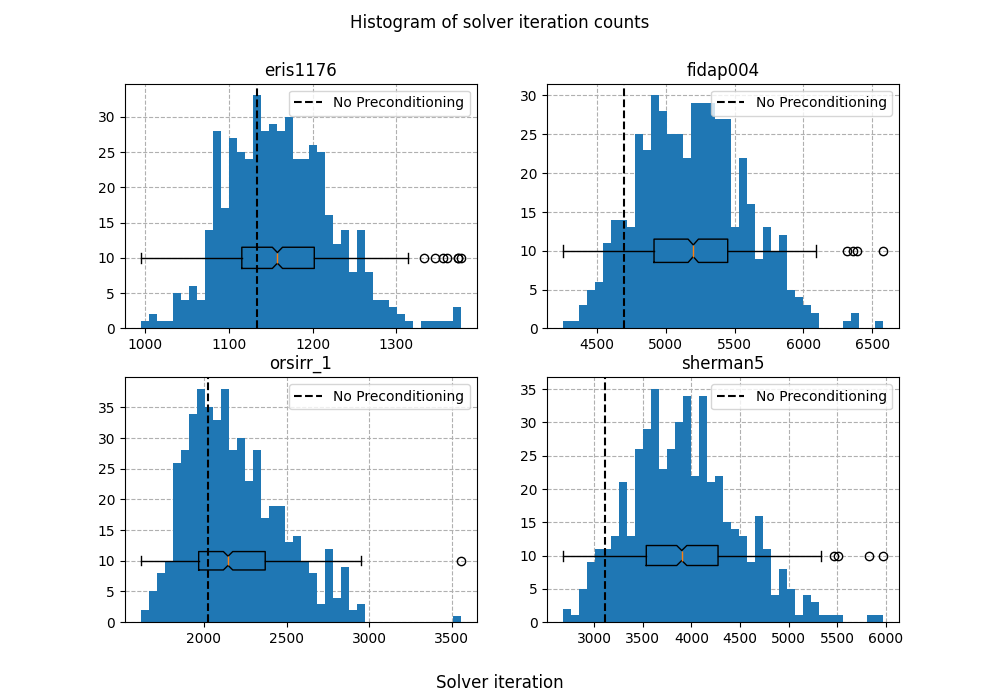
\includegraphics[width=1\textwidth]{plots/initial_par_shift.png}
    \caption{Histogram and boxplot of the solver iterations counts of 500 preconditioned systems for each of the different Matrix Market matrices with a plot for each, with a dashed line corresponding to the unpreconditioned system solver iteration count.}
    \label{fig: initial par shift test}
\end{figure}
\begin{table}[H]
    \center
    \begin{tabular}{|l|r|r|r|r|r|r|}
        \hline
        Matrix & \begin{tabular}{@{}l@{}} Without \\ preconditioning \end{tabular}& Mean & Median & std & \begin{tabular}{@{}l@{}} Number with \\lower iteration count \end{tabular} & Breakdowns\\\hline
        eris1176 & 1134 & 1159.39 & 1157 & 81.85  & 175 & 1\\
        fidap004 & 4695 & 5197.11 & 5200.5 & 384.88 & 47 & 0\\
        orsirr\_1 & 2025 & 2190.75 & 2146 & 287.80 & 163 & 0\\
        sherman5 & 3115 & 3904.15 & 3898.5 & 606.91 & 31 & 5\\\hline
    \end{tabular}
    \caption{Solver iteration count statics of the four matrices preconditioned systems. With each column in order corresponding to the name of the matrix; the solver iteration count for the unpreconditioned system; the mean, median and standard deviation preconditioned solver iteration counts; the number of preconditioned matrices which have a had a solver iteration count lower than the unpreconditioned system; number of preconditioned system that suffered from a breakdown.}
    \label{table: initial par shift stat}
\end{table}
From both the histograms in figure \ref{fig: initial par shift test} and the second to last column of table \ref{table: initial par shift stat}, showing how many of the preconditioned systems had a fewer number of solver iterations, we can see that partitioned shift preconditioner can has the possibility of working as preconditioner given the right coefficients. And that the condition number of the original system plays a part in how well the preconditioner works, as the two matrices with the highest condition number has the fewest number preconditioners that improved the solver iteration count, this a bit unexpected as system with a higher base solve iteration count has larger potential for a improvements. It could also mean that the coefficient generations might have a bad distribution to generate a good preconditioner for these two specific systems. This is where the learning of the preconditioner comes in, because then the initial coefficient should not matter, but only if the initial preconditioner would cause a breakdown of the algorithm to occur.




\subsection{Initial learning algorithm}\label{sec: initial learn}
We will now construct a learning algorithm that can find a set of coefficients for the partitions of the preconditioner such that the preconditioned system have a decreased solver iteration count. Then we will test the algorithm on the four matrices from the previous section. The reason we construct a leaning algorithm and not using an already established Machine Learning algorithm is the need to define a loss function. The standard loss functions expect a continues input, if then we use the solver iteration count as the input to those functions it might run into unexpected behavior. And because the condition number is only a bound for the error it is not the ideal measure of improvement.

The approach we take to learning the coefficients of the preconditioner takes inspiration from stochastic gradient decent. Starting with randomly generated initial coefficients for the partitions with a predetermined number of partitions. Then choose one of the coefficient at random to be change by value generated from some distribution. With this new changed preconditioner the new system is solved to get a solver iteration count to use as a measure, to determine of the change made to the coefficient had a positive or negative effect on the solver iteration. If it decreases the change is kept, otherwise if it increases the iteration count it is rejected. Regardless of the outcome a new coefficient is chosen to be changed. This procedure is then repeated for a number of predetermined learning steps. Pseudocode for this procedure can be seen in Algorithm \ref{alg: initial learn}.

The new parameters that needs to be determined for the learning algorithm is: number of learning steps and how to change the partition coefficients. To choose which coefficient that will be changed we have decided on uniform distribution for which coefficient to be changed, with the knowledge that for larger number of partitions, a larger number of learning steps is needed to explore each coefficient thoroughly. For the value of the change to the coefficient we will use a uniform distribution with mean of zero and different range for each of the four test matrices. Lastly for the number of learning steps we set this to 300 for all test matrices. The number of partitions and the distribution parameters can be seen in table \ref{table: initial learn param}.

\begin{algorithm}
    \caption{Preconditioner learning algorithm}\label{alg: initial learn}
    \begin{algorithmic}
        % \Require $n \geq 0$
        \Require Matrix \(A\) and vector \(b\) form \(Ax=b\)
        \State \(M^{-1} \gets \) Generate initial preconditioner
        \State \(k \gets\) Solver iteration count for \(M^{-1}Ax=M^{-1}b\)
        \Loop{ \(i=1,2,\ldots\)}
            \State \(M^{-1}_{new} \gets \) Changed \(M^{-1}\)
            \State \(k_{new} \gets\) Solver iteration count for \(M^{-1}_{new}Ax=M^{-1}_{new}b\)
            \If{ \(k_{new} < k\)}
                \State \(k \gets k_{new}\)
                \State \(M^{-1} \gets M^{-1}_{new}\)
            \EndIf
        \EndLoop
    \end{algorithmic}
\end{algorithm}


\begin{table}[H]
    \center
    \begin{tabular}{|l|r|r|r|r|}
        \hline
        Matrix &\begin{tabular}{@{}l@{}}Number of\\ partitions\end{tabular}&\begin{tabular}{@{}l@{}}Coefficient\\ distribution\end{tabular} & \begin{tabular}{@{}l@{}}Change\\ distribution\end{tabular}  \\ \hline
        eris1176 & 8 & \(N(0,0.1^2)\) & \(Uni(-0.5,0.5)\)\\
        fidap004 & 8 & \(N(0,0.05^2)\) & \(Uni(-0.1,0.1)\)\\
        orsirr\_1 & 15 & \(N(0.01^2)\) & \(Uni(-1,1)\)\\
        sherman5 & 4 & \(N(0,0.05^2)\) & \(Uni(-0.01,0.01)\)\\\hline
    \end{tabular}
    \caption{The learn parameters for the different matrices with each column corresponding to in order the name of the matrix; number of partitions in the preconditioner; the distribution for the initial partition coefficient; the distribution for the changing the values of the coefficients.}
    \label{table: initial learn param}
\end{table}



\begin{figure}[H]
    \center
    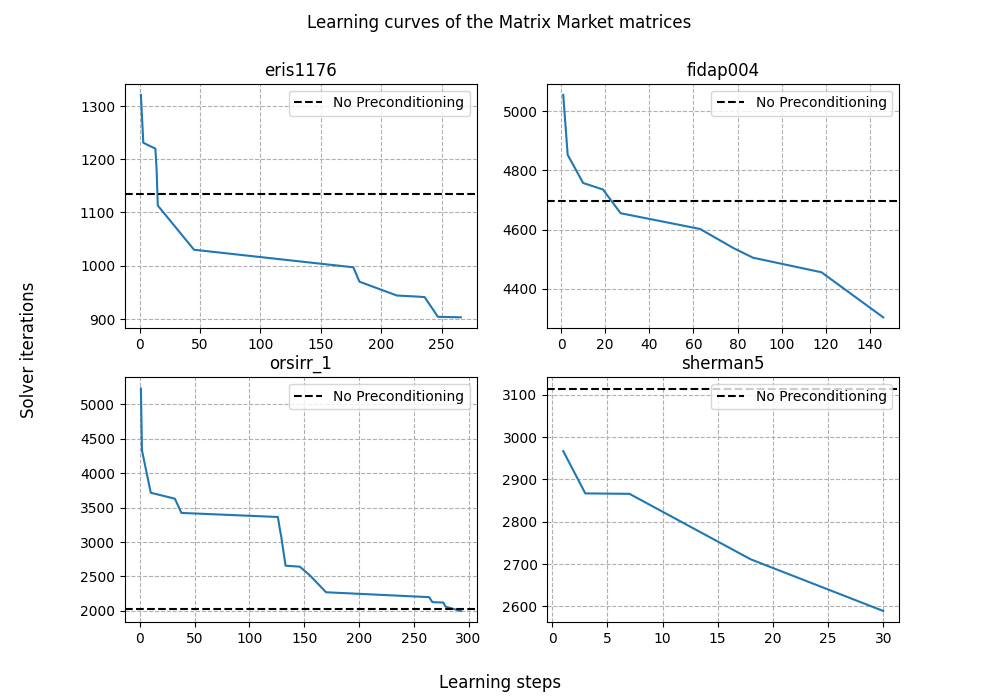
\includegraphics[width=0.8\textwidth]{plots/initial_learn.png}
    \caption{Learning curves of each of the four test matrices. Where the blue line shows the solver iteration count, with data point for each learning step the algorithm accepted a new preconditioner, and a dashed line indicating the unpreconditioned solver iteration count for corresponding matrix.}
    \label{fig: initial learn}
\end{figure}
\newpage
What immediately can be seen from the learning curves in figure \ref{fig: initial learn}, is that our algorithm does what we set out to do.  Because it finds a better set of coefficient that form a better preconditioner and that it uses fewer solver iterations than the corresponding system with a preconditioner applied. The final solver iteration counts can be seen in table \ref{table: initial learn stat}. Another thing, that is not immediately obvious, is that very few of the learning steps a new preconditioner got accepted, at most 17 out the 300 iterations for orsirr\_1 but this may be because of the initial preconditioner making the system much worse and therefore easier to learn. It is difficult to tell if this is a real problem because of the fact the all learned preconditioner works better than with no preconditioner applied, even when the initial preconditioner makes the solver iteration count much larger. The few number of improvements for sherman5 could be contributed to the fact that the initial preconditioner already improves the system and starts at a lower solver iteration count than the unpreconditioned, so it may have learned what it can with few steps. This difficult to say from sherman5's data, but it is clear from the runs for the three other matrices that this learning method can work.

\begin{table}[H]
    \center
    \begin{tabular}{|l|c|c|c|c|}
        \hline
        Matrix & Final & Compare v Non & \begin{tabular}{@{}l@{}}Learning\\ improvement\end{tabular} & \begin{tabular}{@{}l@{}}Number of \\ improvements\end{tabular}\\ \hline
        eris1176 & 903 & 231 & 418 & 14\\
        fidap004 & 4304 & 391 & 750 & 10 \\
        orsirr\_1 & 1998 & 27& 3233 & 17 \\
        sherman5 & 2589 & 526 & 378 & 5 \\\hline
    \end{tabular}
    \caption{Table of data from the learning of the preconditioner with row for each for the matrices and columns corresponding to in order the name of the matrix; the solver iteration count for the final preconditioner; how many fewer solve iterations the preconditioned used compared to the unpreconditioned system; solver iteration count difference between the initial preconditioned system and the final preconditioned system; the number of times a a change to the preconditioned was accepted.}
    \label{table: initial learn stat}
\end{table}


\subsubsection{Better exploration of the preconditioner}\label{sec: better exploration}
As mentioned in the previous section the number of learning steps where a change was accepted. This could be because of a bad exploration of the coefficients in the partitions. The change we will make to the learning algorithm is as such: if a change made to the preconditioner did not improve the solver iteration count, we will try the same change on the same coefficient scaled by \(0.5\), if that worked the scaled change is accepted and continues as the original algorithm. If this scaled change also get rejected, the change will be scaled by \(0.25\). Then if all scaled changes does not improve the solver iteration count the algorithm continues as normal by generating a new change and a new coefficient is chosen. For pseudocode see Algorithm \ref{alg: leaning with scales}. Because the new version of the learning algorithm will test up to 3 times as many different preconditioners, therefore for the test to be comparable to the previous test we will use a base number of learning steps of 100 instead of 300. Other parameters of the algorithm will not be changed, table \ref{table: initial learn param}.

When comparing the result to the previous test the learned preconditioner is a small amount worse and the reason for the change to the algorithm also did not improve as the number of accepted preconditioners is also less, table \ref{table: initial change stat}. A positive improvement is that the learning curves are steeper meaning faster learning, figure \ref{fig: change of scale}. This is especially notable for the matrix fidap004 and might explained the fewer number of improvements. As now the algorithm finds the best preconditioner faster and can therefore find any more changes that would improve the preconditioner. Because the learned preconditioner are only a marginally worse and especially the faster learning, we will keep the change made to the learning algorithm.

\begin{algorithm}[H]
    \caption{Preconditioner learning algorithm with scaling of the change}\label{alg: leaning with scales}
    \begin{algorithmic}
        % \Require $n \geq 0$
        \Require Matrix \(A\) and vector \(b\) form \(Ax=b\)
        \State \(M^{-1} \gets \) Generate initial preconditioner
        \State \(k \gets\) Solver iteration count for \(M^{-1}Ax=M^{-1}b\)
        \Loop{ \( i=1,2,\ldots\)}
            \Loop { \(s=\left\lbrace 1, 0.5, 0.25\right\rbrace\)}
                \State \(M^{-1}_{new} \gets \) Changed \(M^{-1}\) with scale \(s\)
                \State \(k_{new} \gets\) Solver iteration count for \(M^{-1}_{new}Ax=M^{-1}_{new}b\)
                \If{ \(k_{new} < k\)}
                    \State \(k \gets k_{new}\)
                    \State \(M^{-1} \gets M^{-1}_{new}\)
                    \State Break the scale for loop
                \EndIf
            \EndLoop
        \EndLoop
    \end{algorithmic}
\end{algorithm}

\begin{figure}[H]
    \center
    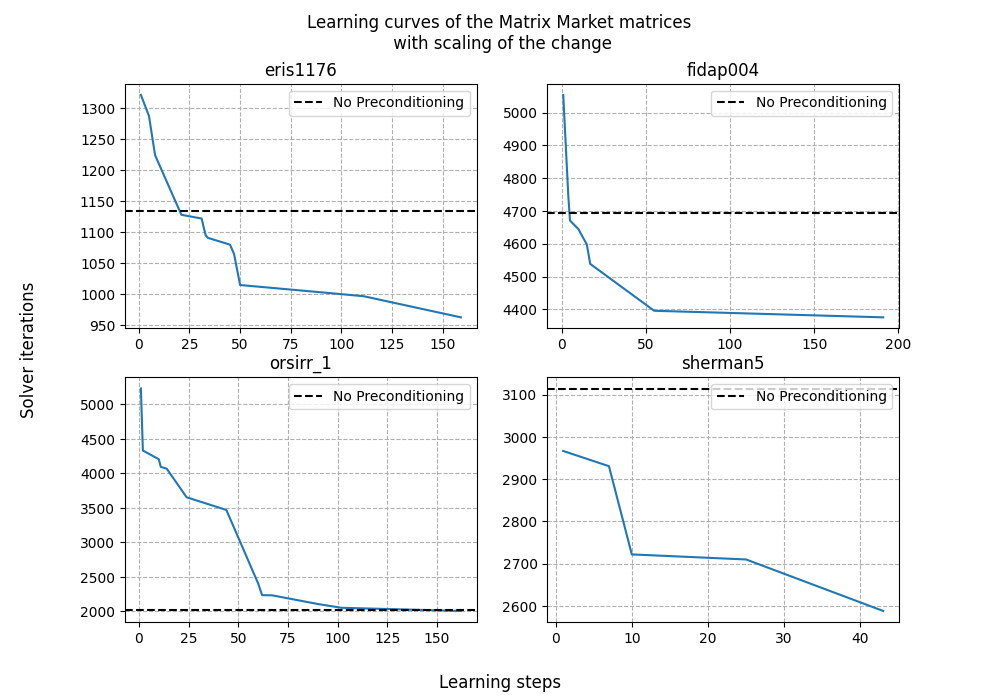
\includegraphics[width=0.8\textwidth]{plots/change_scale.png}
    \caption{Learning curves with scaling the change during learning for the four different test matrices. Where the blue line shows the solver iteration count, with a data point for each learning step the algorithm accepted a new preconditioner, and a dashed line indicating the unpreconditioned solver iteration count for corresponding matrix.}
    \label{fig: change of scale}
\end{figure}

\begin{table}[H]
    \center
    \begin{tabular}{|l|c|c|c|c|}
        \hline
        Matrix & Final & Compare v Non & \begin{tabular}{@{}l@{}}Learning\\ improvement\end{tabular} & \begin{tabular}{@{}l@{}}Number of \\ improvements\end{tabular}\\ \hline
        eris1176 & 963  & 171& 358 & 14 \\
        fidap004 & 4376  & 319& 678 & 8 \\
        orsirr\_1 & 2007  & 18& 3224 & 13 \\
        sherman5 & 2588  & 527& 379 & 5 \\\hline
    \end{tabular}
    \caption{Table of data from the learning of the preconditioner with scaling the change of the preconditioner with a row for each for the matrices and columns corresponds as table \ref{table: initial learn stat}.}
    \label{table: initial change stat}
\end{table}



\subsection{Discrete laplace operator}
The main problem with the two previous tests and how we are using the learning algorithm, is that we only have one linear system for each run of the algorithm. A consequences of this is that the algorithm does not learn a preconditioner that could work for some general matrix, but a good preconditioner for that specific matrix, which is what this project is about. A parallel to this is that with only one matrix the algorithm is unnecessary, as we are learning to solve the system with fewer iteration by solving system itself. The only way to solve this is to get more matrices and to have a set matrices for the training part and set to evaluate the learned preconditioner, as to ensure the algorithm is not overfitting to the training data. To do this we will use the 2-dimensional discrete laplace operator, \(\Delta\), with periodic boundary conditions. As the laplace operator has a direct connection to the Dirac operator \(D^2=\Delta\). 

\noindent The \(D\)-dimensional discrete laplace operator can be constructed as such \cite{boutot2026},

\begin{equation}
    \Delta =\sum_{d=1}^{D}\left(\left(\bigotimes_{k=d}^{d-1} I^{(N_k)} \right)\otimes \Delta_{h_d}^{(N_d)} \otimes \left(\bigotimes_{k=d+1}^{D}I^{(N_k)}\right)\right).
\end{equation}
Where \(\Delta_{h_d}^{(N_d)}\) is the \(N_d\times N_d\) 1-dimensional discrete laplace operator, where we have chosen with periodic boundary conditions, for the \(d\)'th dimension is defined as
\begin{equation}
    \Delta_{h_d}^{(N_d)}=\frac{1}{h_d}
    \begin{bmatrix}
    -2 &1 & 0 &\cdots & 0 & 1\\
    1 & -2 &1 & \cdots & 0 & 0\\
    \vdots&\vdots & \ddots & \vdots & \vdots\\
    0 & 0 &0 & \cdots & -2 & 1\\
    1 & 0 &0 & \cdots & 1 & -2
    \end{bmatrix},
\end{equation}
with discretization step size of \(h_d\) and \(N_d\) grid points. \(I^{(N_d)}\) is a \(N_d\times N_d\) identity matrix. \(A\otimes B\) is the Kronecker product defined between two matrices \(A\) and \(B\) of size \(n\times m\) and \(i\times j\) respectively as

\begin{equation*}
    A\otimes B =
    \begin{bmatrix}
    a_{11} B & \cdots & a_{1m}B\\
    \vdots  & \ddots & \vdots\\
    a_{n1}B & \cdots & a_{nm}B
    \end{bmatrix},
\end{equation*}
and the resulting matrix is of size \(n\cdot i \times m\cdot j\).

\noindent The 2-dimensional laplace can then be written as

\begin{equation}\label{eq: 2d laplace Kronecker}
    \Delta_{h_1}^{(N_1)}\otimes I^{(N_2)} + I^{(N_1)}\otimes \Delta_{h_2}^{(N_2)}.
\end{equation}

Because we want the matrices to be invertible, the matrix has to be square and the Kronecker produces a matrix of size \(n\cdot i \times m \cdot j\), we will use the same discretization for both dimensions, \(N_1=N_2=N\) and for simplicity both of the discretization step sizes will be set to one, \(h_1=h_2=1\). An example with \(N=6\) the 2-dimension discrete laplace operator can be seen in figure \ref{fig: 2d laplace heat map} as a heatmap, with zeros removed for clarity .

\begin{figure}[H]
    \center
    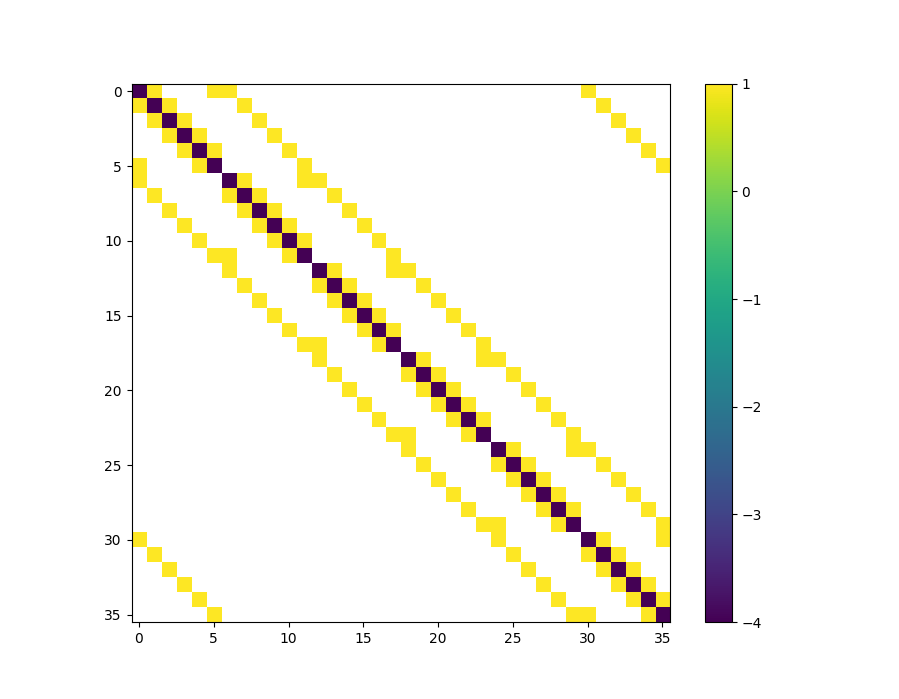
\includegraphics[width=1\textwidth]{plots/2d_laplace_6d1_no_perb.png}
    \caption{2-dimensional discrete laplacian operator with discretization of size \(N_1=N_2=6\) and discretization step size of \(h_1=h_2=1\) for both dimensions show as a heatmap, with zeros removed.}
    \label{fig: 2d laplace heat map}
\end{figure}



% This does not gets us a whole data set of matrices, as mentioned for each matrix entries will have some level of perturbation applied to it.
Because we want sets of distinct matrices, as we need a unique set of matrices for the training and a set for the evaluation of the learned preconditioners. Each nonzero value in the matrices will have some random perturbation applied to it. The simplest way to implement this to perturb the smaller matrices before doing the Kronecker products in equation \ref{eq: 2d laplace Kronecker}. Because the discretization is the same for both dimensions there is only needed to create three unique matrices to get unique entries for the 2-dimensional laplace operator, see equation \eqref{eq: 2d laplace Kronecker perb}. To get small perturbation we use the normal distribution with a mean of 1 and small standard deviation. Note that because the perturbations are done to the smaller matrices and the Kronecker product, the final perturbations will have a distribution of \(N(1,\sigma^2)\cdot N(1,\sigma^2)\). An example of a perturbed matrix can be seen in figure \ref{fig: 2d laplace perp heat map} with an initial perturbation of \(N(1,0.3^2)\).
\begin{equation}\label{eq: 2d laplace Kronecker perb}
    \Delta_{p}\otimes I_{p_1}+ I_{p_2} \otimes \Delta_{p}.
\end{equation}

\begin{figure}[H]
    \center
    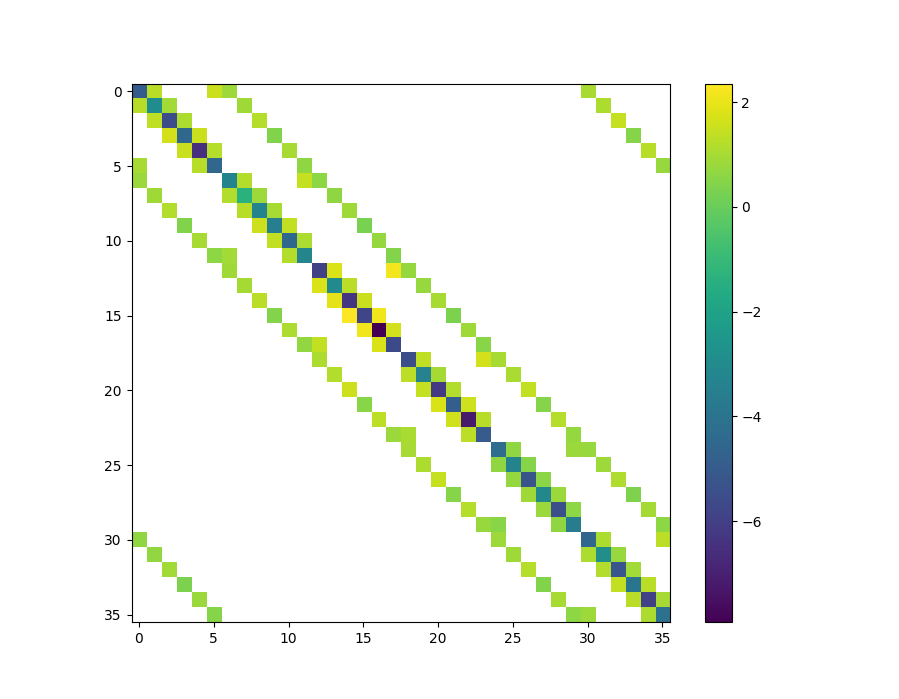
\includegraphics[width=1\textwidth]{plots/2d_laplace_6d1_perp_n_1_0.3.png}
    \caption{2-dimensional discrete laplacian operator with discretization of size \(N_1=N_2=6\) and discretization step size of \(h_1=h_2=1\) for both dimensions with an initial perturbations of \(N(1,0.3^2)\) show as a heatmap, with zeros removed.}
    \label{fig: 2d laplace perp heat map}
\end{figure}

Now that we can generate matrices, we need to determine the parameters of the data generation. These parameters are the discretization size of the 1-dimensional laplace operators and the variance of the initial perturbations. What we would like to have for the solver iteration count is that it is larger than the system size, because then the preconditioner has something to work with. On the other hand we don't want the systems to be too ill-conditioned compared to the size of the system, as we do not want breakdowns to occur for the unpreconditioned linear system, or breakdowns in the exploration of the preconditioner. Therefore we will test four different configurations with 250 matrices each set. The configurations can be seen in table \ref{table: laplace perp param and stat}

\begin{figure}[H]
    \center
    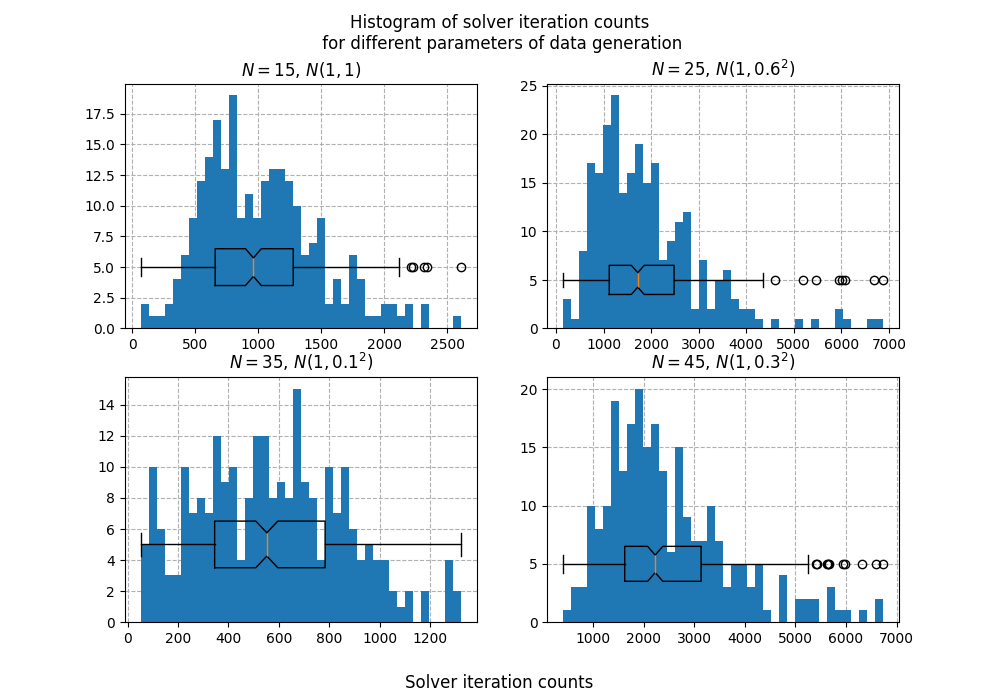
\includegraphics[width=1\textwidth]{plots/laplace_perp_hist.png}
    \caption{Histograms and boxplot of the solver iteration counts for 4 different configurations of the 2-dimensional discrete laplace operator with perturbations, with breakdown occurrences removed.}
    \label{fig: 2d laplace perp hist}
\end{figure}

\begin{table}[H]
    \center
    \begin{tabular}{|l|r|l||r|r|r|r|}
        \hline
        N &\begin{tabular}{@{}l@{}}System \\ Size\end{tabular} & Perturbation & Mean & Median & STD &\begin{tabular}{@{}l@{}}Break \\ downs\end{tabular}\\\hline
        15 &225& \(N(1,1)\) & 1019.1 & 955.5 & 461.11 & 17\\
        25 &625& \(N(1,0.6^2)\) & 1927.6 & 1713 & 1135.8 & 2\\
        35 &1225& \(N(1,0.1^2)\) & 567.2 & 550 & 290.8 & 0\\ 
        45 &2025& \(N(1,0.3^2)\) & 2487.3 & 2218 & 1222.4 & 0\\\hline
    \end{tabular}
    \caption{Parameter configuration and statistic of the four test runs of the 2-dimensional discrete laplace operator with columns corresponding in order to the size of the 1-dimensional discrete laplace operator; the size of the 2-dimensional discrete laplace operator; the initial perturbation distribution; the mean, median, and standard derivation of the solver iterations; the number of systems where a breakdown occurred.}
    \label{table: laplace perp param and stat}
\end{table}

Histograms of the solver iteration count can be seen in figure \ref{fig: 2d laplace perp hist}, and statistic can be seen in table \ref{table: laplace perp param and stat}. The first thing to notice from these four tests is the effect of the perturbations variance has on the solver iteration count. It has a clear positive corelation, meaning with larger variance, the solve iteration count is increased, to the point of becoming too ill-conditioned compared to the system size. This can be seen for configuration with \(N=15\) and perturbation distribution of \(N(1,1)\). What can not be seen in the histograms, because system that had a breakdown occur are removed for readability of the histogram, is that the breakdown that occurred at the latest happened at solver iteration 67337. This is a problem both because that data point is useless for the analysis of the a potential preconditioner, but also because the solving of each of the systems is done in parallel meaning if one of the system take 6 times as long to solve, each learned step has to wait on the that system to breakdown or be solved before it can continues with the learning. Then if the perturbations are smaller, as is the case for the configuration \(N=35\) and \(N(1,0.1^2)\), the solver iteration count are also smaller compared to the size of the system, to the point that a potential preconditioner has very few solver iteration count to improve on. For these reason we will go forward with with the last of the configurations with \(N=45\) and \(N(1,0.3^2)\), as the median solver iteration count is larger than the system size, most iteration count are larger than the system size without having any systems with an occurrences of a breakdown.

With the generation of data the procedure for learning and evaluation of the preconditioners needs to be changed. For each of the learning tests two sets of matrices will be generated of equal amount, one set to be used in the learning of the preconditioner and the other for the evaluation of the learned preconditioner. With this we will avoid overfitting the preconditioner, as the learning algorithm did in the two previous sections \ref{sec: initial learn} and \ref{sec: better exploration}. In the learning algorithm we need a function to determine when a changed is made to the preconditioner was an improvement or if the changed made the preconditioner worse, this we call the improvement function. The functions will be defined and tested in the next section \ref{sec: Improve func}. In the evaluation of the learned preconditioner we will look at three different measures to determine if the preconditioner is good. The first two is the mean and median solver iteration count of the preconditioned system, this will compared against mean and median solver iteration count of the linear systems solved without a preconditioner applied. The third measure will count how many individual systems where the preconditioner reduced the solver iteration compared with using no preconditioner.


\subsection{Improvement functions}\label{sec: Improve func}
As mentioned in the previous section we need a function to determine if changed made to the preconditioner was an improvement. Because this part of the algorithm is especially important, we will test three different improvement functions, for four different seeds each. The improvement functions will described in the following subsections.

\subsubsection{MEAN improvement function}
The first improvement function is the MEAN improvement function. It will accept a change made to the preconditioner if the mean solver iteration count of the preconditioned systems is lower than the previous mean solver iteration count.
\subsubsection{MEDIAN improvement function}
The second improvement function is the MEDIAN improvement function. It will accept a change made to the preconditioner if the median solver iteration count of the preconditioned systems is lower than the previous median solver iteration count.
\subsubsection{SIGN improvement function}
The last improvement function is the SIGN improvement function. It will accept a change made to the preconditioner if a majority of the preconditioned systems have a decreased solver iteration count compared with solver iteration count using the unchanged preconditioner. The name comes from the implementation where a difference of the individual systems solver iteration counts, then it counts the number of occurrences with negative sign and positive sign.

One problem that might occur with the SIGN improvement function is: on a data set with 100 linear systems. If 55 of the systems have a reduction of 1 solver iteration count with the changed preconditioner, and the last 45 have an increase of 1000 solver iteration counts with the changed preconditioner. This new preconditioner would be accepted by the SIGN improvement function. But with this new preconditioner could have both an increase in mean and median solver iteration count. Therefore would not be accepted by the other two improvement functions. How likely for such a state similar to this example is to occur and if the changes are as big as the given example, is to be determined by the testing of the improvement function.

Another point to consider is what to do when change to the preconditioner makes one or more of the systems have a breakdown occur, as this could drastically change the solver iteration count of the system in either direction and skew all three of the improvement functions measure. We could remove the data point from the improvement measure, but this would still change result of the improvement function. Because if system with previous largest iteration count had a breakdown the mean and median would be smaller and for the SIGN improvement function needs to data sets of equal size to make the decision. For these reasons we will also add the condition that all preconditioned systems must converge for a change to the preconditioner to the accepted. This could cause problem if a system starts ill-conditioned or if the initial coefficient of the preconditioner are bad. The new version of the algorithm see algorithm \ref{alg: leaning with improvement function}.


\begin{algorithm}
    \caption{Preconditioner learning algorithm with improvement functions.}\label{alg: leaning with improvement function}
    \begin{algorithmic}
        % \Require $n \geq 0$
        \Require A set of matrices and vectors than each form a linear system \(A_ix=b_i\)
        \Require An improvement function \(f\)
        \State \(M^{-1} \gets \) Generate initial preconditioner
        \State \(k\_list \gets\) A list of solver iteration count for each \(M^{-1}A_ix=M^{-1}b_i\)
        \Loop{ \( i=1,2,\ldots\)}
            \Loop { \(s\in \pm\left\lbrace 1, 0.5, 0.25\right\rbrace\)}
                \State \(M^{-1}_{new} \gets \) Changed \(M^{-1}\) with scale \(s\)
                % \State \(k\_list_{new} \gets\) Solver iteration count for \(M^{-1}_{new}Ax=M^{-1}_{new}b\)
                \State \(k\_list_{new} \gets\) A list of solver iteration count for each \(M^{-1}_{new}A_ix=M^{-1}_{new}b_i\)
                \If{ \(f\) accepts the new state \textbf{and} all systems converged}
                    \State \(k\_list \gets k\_list_{new}\)
                    \State \(M^{-1} \gets M^{-1}_{new}\)
                    \State Break the scale for loop
                \EndIf
            \EndLoop
        \EndLoop
    \end{algorithmic}
\end{algorithm}


The other run parameters will be the same for all 12 test,  see table \ref{table: improvement func test config}. The choice of the parameters are made from the conclusions from the previous sections tests. With a change to the list of scales \(\pm \left\lbrace 1,0.5,0.25\right\rbrace\) as to explore both directions of the possible change to the coefficient. Another change compared to the initial learning in section \ref{sec: initial learn} the step of the algorithm that solves the systems with Bi-CGStab will be done in parallel.

\begin{table}
    \center
    \begin{tabular}{|r|r|r||r|r||r|r|}
        \hline
        \(N\) & Perturbation & Amount &\begin{tabular}{@{}l@{}}Base learn \\steps\end{tabular} & Learn Scales & \begin{tabular}{@{}l@{}}Initial\\coefficient\\distribution\end{tabular} & \begin{tabular}{@{}l@{}}Number of\\partitions\end{tabular} \\\hline
        45 & \(N(1,0.3^2)\) & 250 & 100 & \(\pm\{1,0.5,0.25\}\) & \(N(0,0.05^2)\) & 10\\ \hline
    \end{tabular}
    \caption{Run parameter configuration. The columns corresponds to in order: the size of the 1-dimensional discrete laplace operator; the initial perturbations; the amount of matrices in each of the data sets; the base number of learning iteration; the scales each change will attempt with; the initial coefficient distribution; the number of partition in the preconditioner.}
    \label{table: improvement func test config}
\end{table}

\begin{figure}[ht]
    \center
    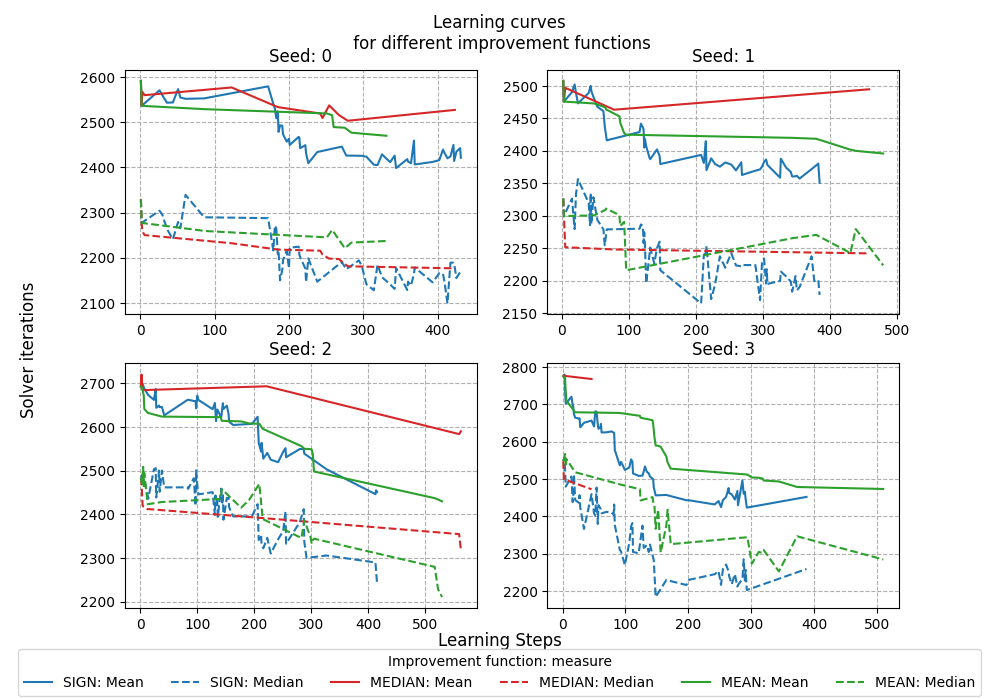
\includegraphics[width=1\textwidth]{plots/improv_func_learn_curve.png}
    \caption{Learning curves for all 12 run configurations. Each plot corresponds to a different seed. The colour of the lines corresponds to a different improvement function: blue for SIGN improvement function; red for MEDIAN improvement function; green for MEAN improvement function. The whole lines is the mean solver iteration count in each learning iteration and the dashed is the median solver iteration count.}
    \label{fig: initial improv learn curve}
\end{figure}

Starting with the MEDIAN improvement function we see from its learning curves in figure \ref{fig: initial improv learn curve}, that it had hard time finding any changes to the preconditioner that would improve the median solver iteration count, with at most 12 accepted preconditioners for seed 0 and down to 3 accepted for seed 3. Table \ref{table: improve func test improvement count} for all acceptance counts. Because of the few number acceptances the evaluation of the preconditioner on the test matrices set, preforms worse in all three measures compared to two other improvement functions for all seeds. Comparing to the unpreconditioned systems the mean and median solver iteration count values are very similar, figure \ref{fig: initial improv test measure}, and only about a fourth of the system have a lower iteration count, figure \ref{fig: initial improv BvN}. With this we can say that the using MEDIAN improvement function in learning does not work. 
\newpage

With MEAN improvement function the problem of few acceptances is not as prevalent, but still happened for seed 0 with 9 instances of improvement occurring. Of the four runs with MEAN improvement function seed 0 is the one that worst in the evaluations of the learned preconditioner mean and median solver iteration count. While int the individual comparison almost a three fourths of the systems have a lower iteration count compared to the unpreconditioned systems for all four seeds. For the other three seeds the learned preconditioners does decrease the solver iteration counts. 

Lastly with SIGN improvement function does not suffer from the problem with few number of improvements, and therefore consistently have a better evaluation of the learned preconditioners. The fluctuations in the learning curves is because of the problem described earlier. From this we can conclude that a preconditioner with this bidiagonal structure can be learned to improve the solver iteration count for an unseen linear systems, with the right improvement function.


\begin{table}[H]
    \center
    \begin{tabular}{|r|r|r|r|}
        \hline
        Seed &SIGN& MEDIAN & MEAN  \\\hline
        0  & 56& 12 & 9 \\
        1  & 60& 5 & 14 \\
        2 & 52 & 7 & 22 \\
        3 & 64& 3 & 25  \\\hline
    \end{tabular}
    \caption{Number of instances a change made to the preconditioner got accepted. A row for each the four seed and columns for each of the three improvement functions.}
    \label{table: improve func test improvement count}
\end{table}



\begin{figure}[H]
    \center
    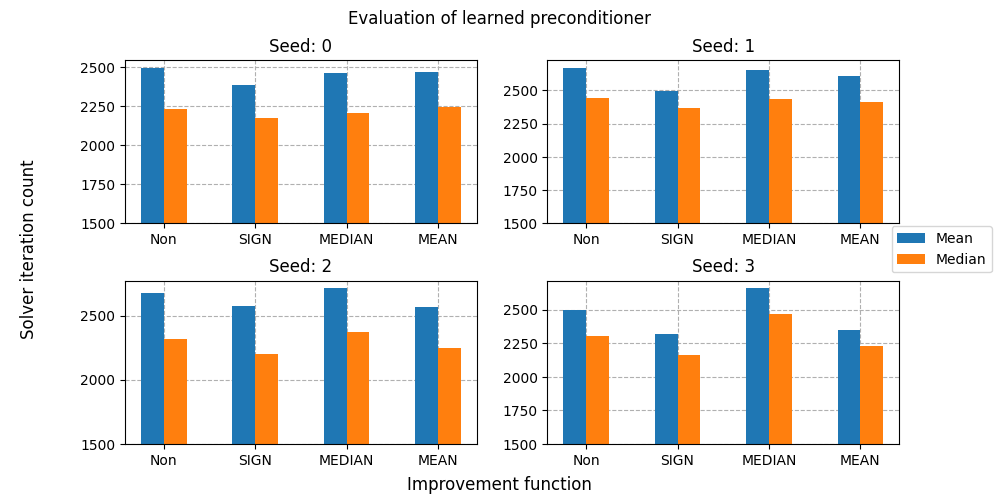
\includegraphics[width=1\textwidth]{plots/improv_func_test_measure.png}
    \caption{Comparison plot of the evaluation of the learned preconditioner where each plot corresponds to a different seed in the learning. The colour of the bars corresponds to the mean solver iteration  count for blue and median solve iteration count for orange. The groups is the different improvement functions used in learning which are in order the unpreconditioned system; SIGN improvement function; MEDIAN as the improvement function; MEAN as the improvement function. Lower is better.}
    \label{fig: initial improv test measure}
\end{figure}



\begin{figure}[H]
    \center
    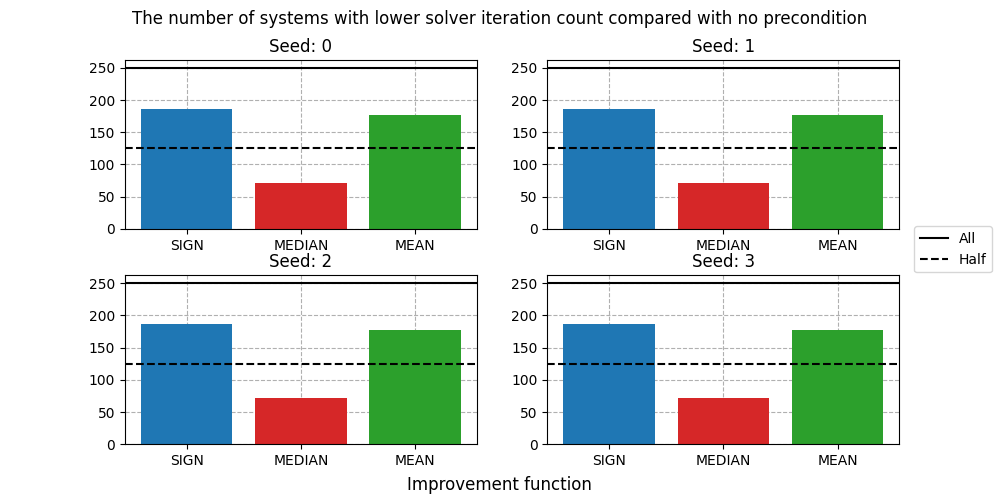
\includegraphics[width=1\textwidth]{plots/improv_func_BvN.png}
    \caption{Bar plot of of many of the system where the preconditioner improved the solver iteration count compared to the unpreconditioned systems. Each plot is for a different seed. The bars corresponds to a different improvement function used in learning indicated by its label. The dashed line is half the data set and full is the whole data set. Higher is better.}
    \label{fig: initial improv BvN}
\end{figure}



\subsubsection{Comparison with Jacobi preconditioning}
For a better comparison of the learned preconditioners, the evaluations should be compared against already know working preconditioner. Because we have information about the structure of the matrices we want to precondition, that is the largest absolute value are on the diagonal and these values do  not equal to 1 or 0. Therefore a good choice of preconditioner is the Jacobi preconditioner, as mentioned in section \ref{sec: prelim precond}. This preconditioner uses the diagonal elements of a matrix as the preconditioner, \(M=diag(a_{11},a_{22},\ldots)\) for matrix \(A=(a_{i,j})\) and therefore a trivial to compute inverse. Preconditioning the test data with the Jacobi preconditioner and using this set of solver iteration counts as the point of comparison for the learned preconditioner. 

What we get from that is the Jacobi preconditioner is better than all learned preconditioners regardless of improvement function and seed, as the mean and median solver iteration count is lower for all four seeds, figure \ref{fig: initial improv test measure with jacobi}. On the individual system level comparison there are systems where the learned preconditioner has lower solver iteration counts, at most 44 systems for seed 1 and SIGN improvement function, figure \ref{fig: initial improv BvJ}. We conclude from this is that our learned preconditioner can still work, but that the current algorithm or preconditioner needs to be changed.


\begin{figure}[H]
    \center
    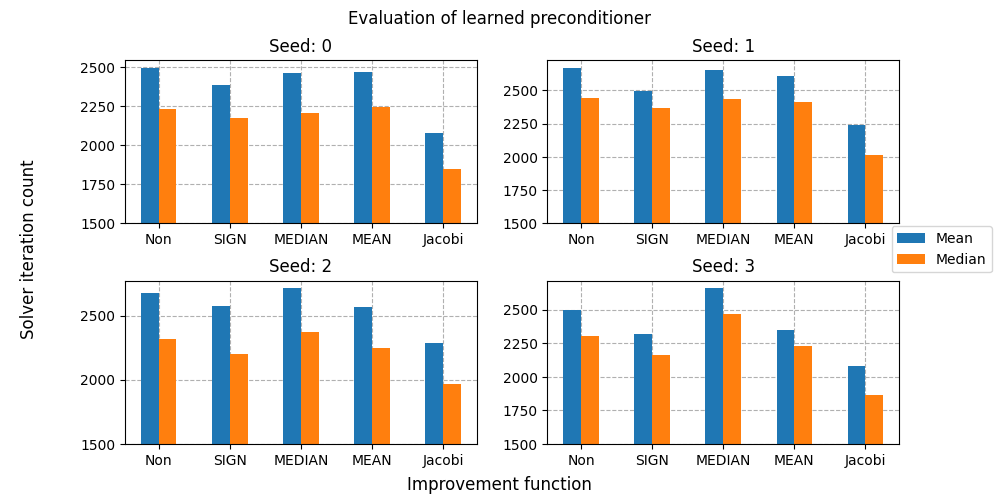
\includegraphics[width=1\textwidth]{plots/improv_func_test_measure_jacobi.png}
    \caption{The same plot as figure \ref{fig: initial improv test measure} with a bar group added for the mean and median solver iteration count for the systems preconditioned with the Jacobi preconditioner.}
    \label{fig: initial improv test measure with jacobi}
\end{figure}

\begin{figure}[H]
    \center
    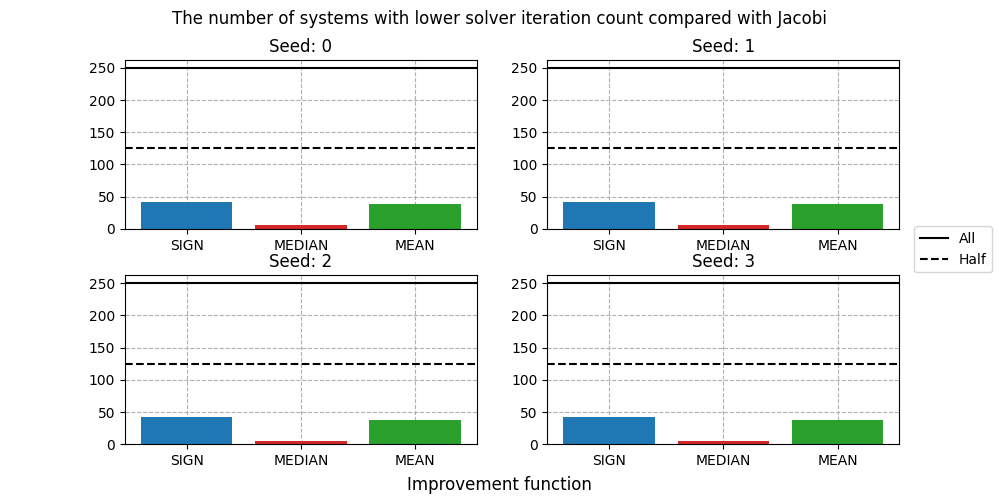
\includegraphics[width=1\textwidth]{plots/improv_func_BvJ.png}
    \caption{A similar plot to figure \ref{fig: initial improv BvN} with the difference of instead of comparing the solver iteration count to the unpreconditioned system it is compared to the systems preconditioned with Jacobi preconditioner.}
    \label{fig: initial improv BvJ}
\end{figure}


\newpage
\subsection{Shifted Jacobi preconditioner}\label{sec: jacobi shift}
The change we will make is to the structure of the partition shift preconditioner is replacing the diagonal of the matrix from the identity to inverse of the diagonal of the matrix it is applied to. Meaning combining Jacobi preconditioning and our partition shift preconditioner to get a new preconditioner we will call Shifted Jacobi preconditioner. This means our new preconditioner consistent of system specific part, the main diagonal, and a general learned part, the partitioned superdiagonal. A constraint that the new preconditioner has for the matrix it is applied to is that all diagonal entries of the matrix has to have a nonzero value. 

To test this new preconditioner we will run the learning algorithm with the same parameters as the previous test in section \ref{sec: Improve func} table \ref{table: improvement func test config}, with the only change being the preconditioner.

\begin{table}[H]
    \center
    \begin{tabular}{|l|r|r|r|}
        \hline
        Seed &SIGN& MEDIAN & MEAN  \\\hline
        0 & 39 & 25 & 29 \\
        1 & 37 & 27 & 23 \\
        2 & 58 & 27 & 26 \\
        3 & 65 & 37 & 34 \\\hline
    \end{tabular}
    \caption{Number of times a new preconditioner was accept. A row for each seed and column for each improvement function.}
    \label{table: Jacobi par shift improvement count}
\end{table}

\begin{figure}[H]
    \center
    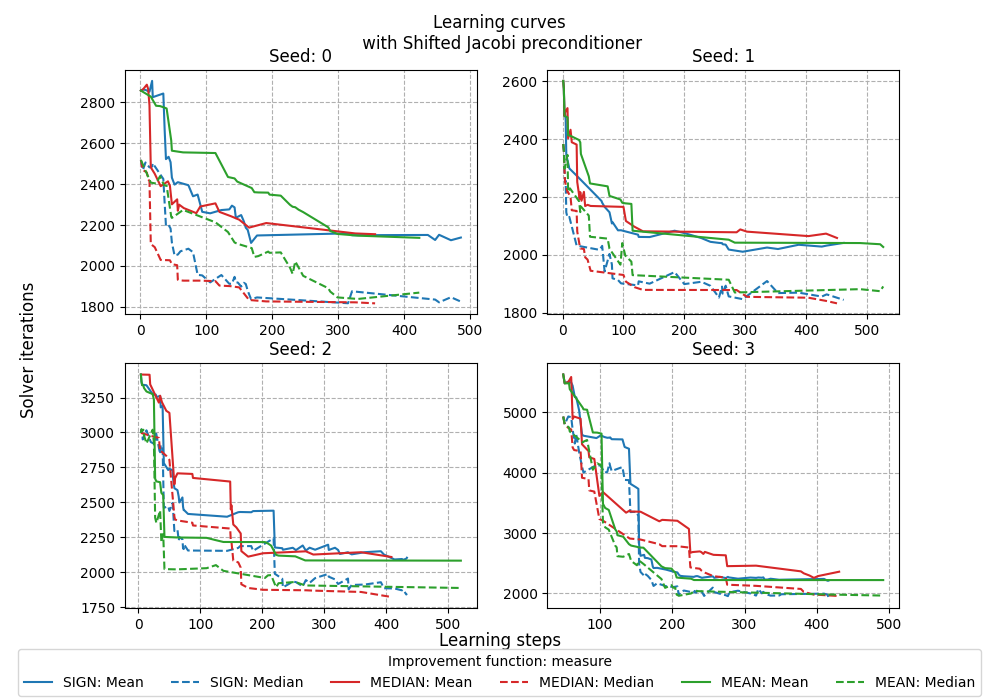
\includegraphics[width=1\textwidth]{plots/jacobi_par_shift_learning_curve.png}
    \caption{Learning curves for testing Shifted Jacobi preconditioner. The plot has the same structure as figure \ref{fig: initial improv learn curve}, a plot for each seed, colours indicate improvement function, and line style corresponds to solver iteration count mean or median.}
    \label{fig: Jacobi par shift learning curves}
\end{figure}


From the learning curves in figure \ref{fig: Jacobi par shift learning curves}, we can see clear improvements when comparing to the learning curves from the previous tests in figure \ref{fig: initial improv learn curve}. The mean and median solver iteration count decrease significant amount during the learning for all three improvement function, where as before with MEDIAN improvement function had difficulty finding improvements to the preconditioner. Even when the initial preconditioner starts with mean solver iteration count above 5000 for seed 3 and the final iteration counts is only a bit higher compared to the other seeds, but this may be because the data set and not the preconditioner. 

Another improvement is the number of accepted coefficient changes made during learning is considerably larger for MEAN and MEDIAN improvement functions and similar for SIGN, table \ref{table: Jacobi par shift improvement count}, again comparing to the previous learning tests in section \ref{sec: initial par shift}. This means that even before looking at the evaluation, we can expect the learned preconditioners being good. And lastly a new problem has occurred from the learning curves is that it looks like the learning has plateaued, example for seed 1 the amount of change that happens to the mean and median solver iteration count after learning step 150 is minimal compared to the earlier leaning step. This could mean that it has found the best preconditioner, that it has found a local minimum and the changes made to the preconditioner are not big enough to find a better minimum, or that it did not have enough steps iteration and not plateaued.

In the evaluations of the preconditioner on the test data, there is only a marginal improvement compared to Jacobi preconditioning on its own for the mean and median solver iteration counts, figure \ref{fig: jacobi par shift test measure}, and only with SIGN and MEAN improvement functions we get more than half of the systems having a lower solver iteration count than when using Jacobi preconditioning, figure \ref{fig: Jacobi par shift BvJ}. For the differences in improvement function there is very little difference in the evaluations of the learned preconditioners, with SIGN being slightly better across all the seeds for this reason and because it worked the best in the previous test we will only use the SIGN improvement function for all further testing of the learning algorithm and structural changes to the preconditioner. From this it is easy to say that these learned preconditioners with Jacobi diagonal are better than the previous learned preconditioners with identity diagonal, but only slightly better than the simple Jacobi preconditioning.


\begin{figure}[H]
    \center
    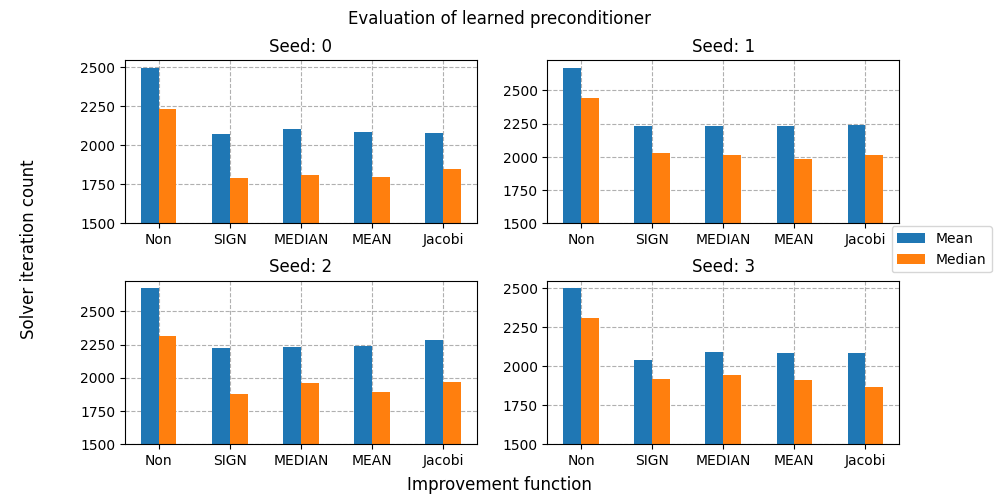
\includegraphics[width=1\textwidth]{plots/jacobi_par_shift_test_measure.png}
    \caption{Evaluation of the learned preconditioners with the same structure as figure \ref{fig: initial improv test measure with jacobi}. A plot for each seed, with a bars for the three improvement functions and 2 to compare with unpreconditioned and Jacobi preconditioned solver iteration count. Bar colours indicate mean (blue) and median (orange) solver iteration count.}
    \label{fig: jacobi par shift test measure}
\end{figure}

\begin{figure}[H]
    \center
    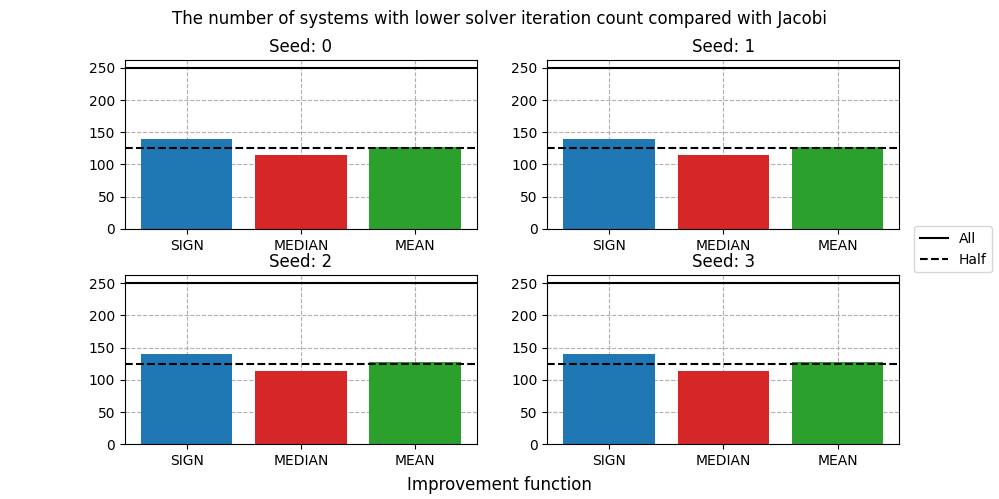
\includegraphics[width=0.95\textwidth]{plots/jacobi_par_shift_BvJ.png}
    \caption{Individual system comparison plot with the same structure as \ref{fig: initial improv BvJ}. A plot for each seed, bars for each improvement function, and lines to indicate all or half the systems.}
    \label{fig: Jacobi par shift BvJ}
\end{figure}




\subsubsection{Plateau in learning}\label{sec: plateau}
As mentioned the previous tests learning curves semed to have plateaued. Therefore we will run the configuration from the previous test with seed 0 and the SIGN improvement function with 500 base learning steps. This is to see if the learning did plateau. If that is the case the solver iteration counts should stay relatively unchanged. Or if the algorithm could find a better preconditioner after the base 100 learning steps from the previous test.

What we get from the learning curve in figure \ref{fig: plateau learning curves} is that the learning has plateaued and no significant changes are made after 500th learning step. The fluctuations is inherent to the SIGN improvement function, which has been mentioned earlier. In the evaluation of the learned preconditioner there is no significant differences between the run with 100 and 500 base learning steps, having only slightly higher mean and median solver iteration counts, this is because in the current version of the algorithm the learned preconditioner is the last version in learning, meaning because of the fluctuations it ended in with a slightly worse preconditioner.

\begin{figure}[H]
    \begin{minipage}{.49\textwidth}
        \center
        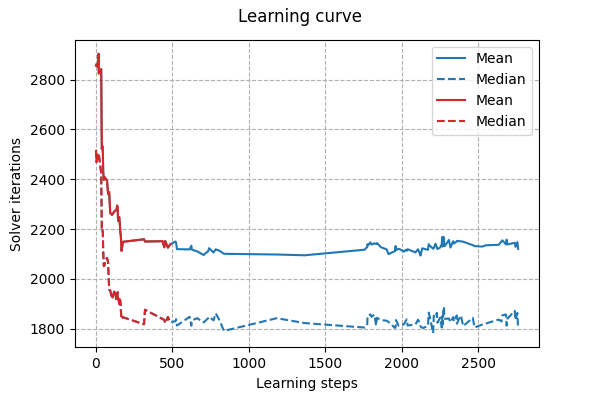
\includegraphics[width=1\textwidth]{plots/plateau_learning_curve.png}
        \caption{Learning curve for seed 0 and SIGN improvement function with 100 base learning iterations, red curve, and 500 base learning iterations, blue curve. Line style indicate mean (full line) and median (dashed line) solver iteration count.}
        \label{fig: plateau learning curves}
    \end{minipage}
    \begin{minipage}{.02\textwidth}
        
    \end{minipage}
    \begin{minipage}{.49\textwidth}
        \center
        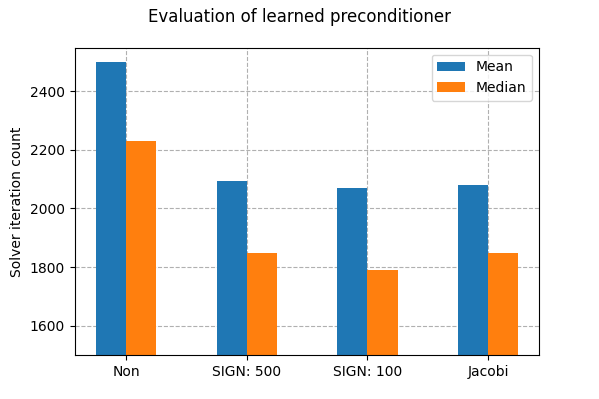
\includegraphics[width=1\textwidth]{plots/plateau_test_measure.png}
        \caption{Evaluation of the learned preconditioner, with the same structure as figure \ref{fig: jacobi par shift test measure}, for the run with seed 0 and SIGN improvement function with 100 and 500 base learning iterations.\\}
        \label{fig: plateau test measure}
    \end{minipage}
\end{figure}


\subsection{Allowing disimprovement}
To try overcoming the problem of the algorithm plateauing the learning, we will change the learning algorithm such that it can allow changes made to the coefficients to be accepted, even when the improvement function would have decided to rejected the change. We do this because we suspect that the preconditioner is an local minimum, and hope by accepting these changes to find a better minimum. The acceptance of a worse state will be done be with a probability that is inverse proportional to how much worse the change is making the new preconditioner, as to not accepted every change made. Where worse is defined by the improvement function.

Meaning with the SIGN improvement function for a total of 100 matrices: if 45 preconditioned systems solver iteration count decreased and 55 increased it will have a acceptance probability of \(\frac{1}{(55-45)+2}=\frac{1}{12}\). The \(+2\) is there for two reasons, first a \(+1\) to ensure no zero division when an equal amount of system have a decrease and increase in solver iteration count, and second another \(+1\) is add such that not all of these changes where this happens will be accepted. The updated pseudocode can be seen in Algorithm \ref{alg: leaning with disimprovement}. This implementation might need adjustment because the probability is also proportional to the total number of matrices. If the data set is small the probability of accepting a state where all system solver iterations count increase would be larger than if the data set was bigger. There is still the condition that all system must converge for any state to be accepted. To test this change to the learning algorithm the same configuration as the runs form the previous section.

From the learning curves in figure \ref{fig: disimprove learning curves} and the evaluation of the learned preconditioners in figure \ref{fig: disimprove test measure} and \ref{fig: disimprove BvJ}, we can see that we gets a slight improvement of the learned preconditioners, meaning we will keep it allowing disimprovements. A thing that was overlooked in the implementation of the disimprovement in the learning algorithm, is that the resulting preconditioner comes from the last accepted learning iteration, meaning that the best found preconditioner is most likely not the preconditioners the algorithm gives as the output. For example if the learning had stopped at solver iteration count spike at learning iteration around 1250, we would have naively concluded that allowing disimprovement is much worse.


\begin{algorithm}[H]
    \caption{Preconditioner learning algorithm with with disimprovement}\label{alg: leaning with disimprovement}
    \begin{algorithmic}
        % \Require $n \geq 0$
        \Require A set of matrices and vectors than each form a linear system \(A_ix=b_i\)
        \Require An improvement function \(f\)
        \State \(M^{-1} \gets \) Generate initial preconditioner
        \State \(k\_list \gets\) A list of solver iteration count for each \(M^{-1}A_ix=M^{-1}b_i\)
        \Loop{ \( i=1,2,\ldots\)}
            \Loop { \(s\in \pm\left\lbrace 1, 0.5, 0.25\right\rbrace\)}
                \State \(M^{-1}_{new} \gets \) Changed \(M^{-1}\) with scale \(s\)
                \State \(k\_list_{new} \gets\) A list of solver iteration count for each \(M^{-1}_{new}A_ix=M^{-1}_{new}b_i\)
                \If{all systems converged}
                    \If{\(f\) accepts the new state \textbf{or} with probability accept a worse state}
                        \State \(k\_list \gets k\_list_{new}\)
                        \State \(M^{-1} \gets M^{-1}_{new}\)
                        \State Break the scale for loop
                    \EndIf
                \EndIf
            \EndLoop
        \EndLoop
    \end{algorithmic}
\end{algorithm}

\begin{figure}[H]
    \center
    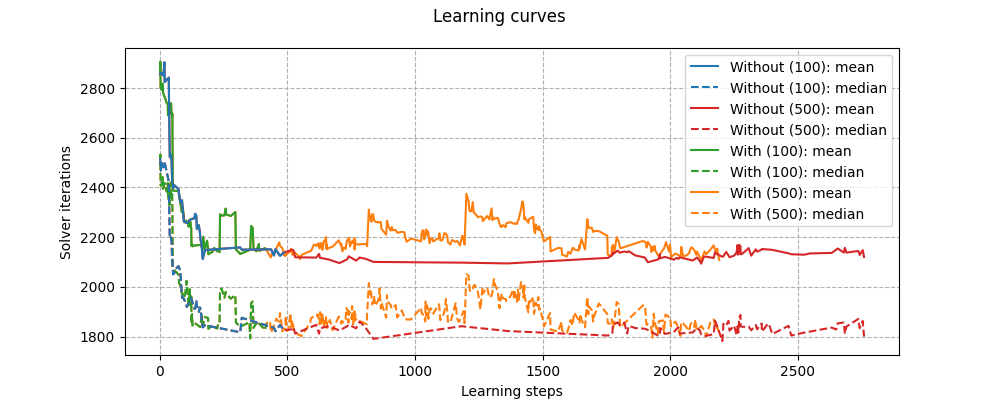
\includegraphics[width=1\textwidth]{plots/disimprove_learn_curve.png}
    \caption{Learning curves for the testing disimprovement where the blue and red lines corresponds to runs without disimprovement with 100 and 500 base learning iterations, this is the same data as in figure \ref{fig: plateau learning curves}, green and orange lines are with disimprovement with 100 and 500 base learning iterations, the new test. Line style corresponds to whole line for the mean and dashed line for the median solver iteration count.}
    \label{fig: disimprove learning curves}
\end{figure}

\begin{figure}[H]
    \center
    \begin{minipage}{.49\textwidth}
        \center
        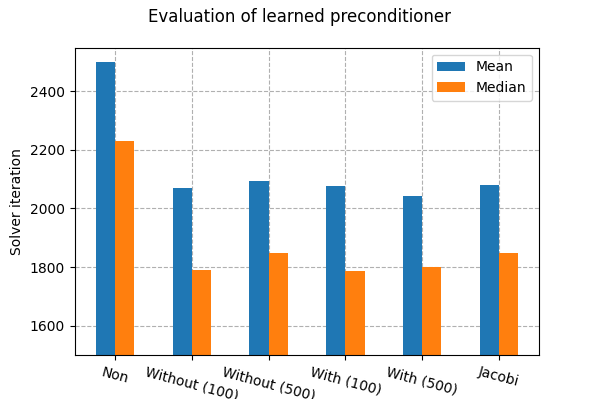
\includegraphics[width=1\textwidth]{plots/disimprove_test_measure.png}
        \caption{Mean and median solver iteration count for the evaluation of the learned preconditioner. Colour indicate measure: Blue is mean and orange is median solver iteration count. A bar group for each of the four tests: without disimprovement with 100 and 500 base learning iterations and with disimprovement with 100 and 500 base learning iteration. On either end the unpreconditioned and Jacobi preconditioned systems for comparison.}
        \label{fig: disimprove test measure}
    \end{minipage}
    \begin{minipage}{.02\textwidth}
        
    \end{minipage}
    \begin{minipage}{.49\textwidth}
        \center
        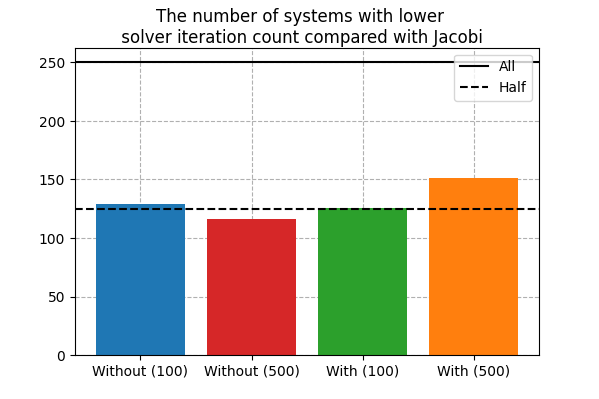
\includegraphics[width=1\textwidth]{plots/disimprove_BvJ.png}
        \caption{Individual linear system comparison between the learned preconditioners and Jacobi preconditioners with bar size corresponding to the number of systems where the learned preconditioner has a lower solver iteration count that Jacobi Preconditioning.\\\\\\}
        \label{fig: disimprove BvJ}
    \end{minipage}
\end{figure}


To resolve this problem the algorithm should keep tack of the best seen preconditioner. Here we would like to again use the improvement function as a measure for which were the best, but the SIGN improvement function can not do comparisons across multiple solver iteration count data sets. Therefore we will use the discarded improvement functions mean and median in combination to determine which accepted preconditioner was the best, as these measure are the measures we look at to determine if the learned preconditioner are good in the evaluation. This measure of best will be done after a new preconditioner have been accepted.



\subsection{Number of partitions}\label{sec: num par}
Because of the results from the previous test, allowing disimprovement, did not improve the learned preconditioner by any significant degree. Therefore we will go back to looking at the structure of our preconditioner. When initial explaining the structure of the Preconditioner, in section \ref{sec: initial par shift}, in the part about the number of partitions of the superdiagonal. We said that with higher number of partitions could lead to a better preconditioner, but with a longer learning time. Therefore the next test will test for larger amount of partitions and the number of partitions we will test is \(\{15,20,25,30,40,50\}\). To compensate for the potential longer learning time these test will also have an increased base number of learning steps from 100 to 200.

The first thing to notice from the learning curves in figure \ref{fig: more par learning curves}, is that our assumption that having more partitions will equate to longer learning is correct. It can most notable be seen in the test with 50 partition, brown learning curve, as the mean and median solver iteration count does go down but at a slower rate compared to the smaller number of partitions. Starting with a mean solver iteration count of 3086 and decreases it to 2332.3 at learn step 248, but then the solver iteration counts does not change by any substantial amount after that. Compared to the run with 15 partitions gets below a mean solver iteration count 2250 at learn step 138, which means that more partitions have slower learning and it plateaus at higher solver iteration counts.


\begin{figure}[H]
    \center
    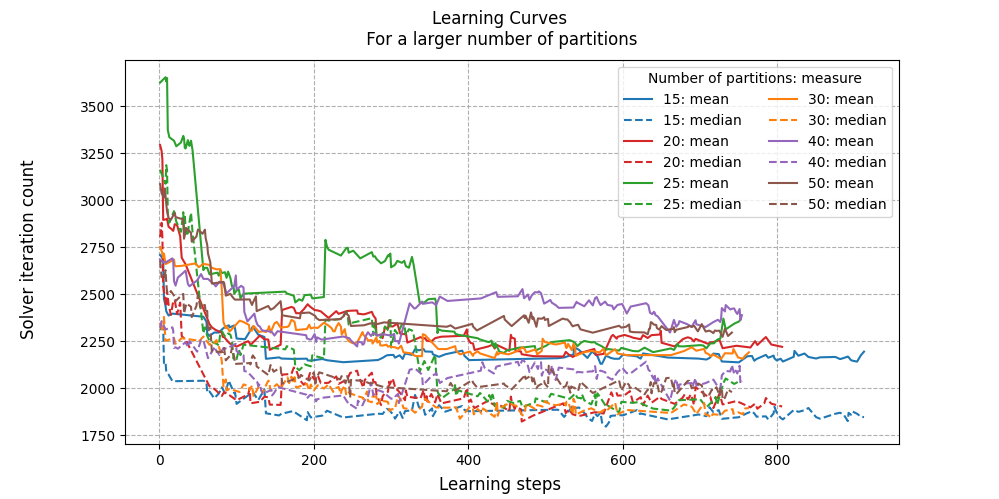
\includegraphics[width=1\textwidth]{plots/more_num_par_learning_curve.png}
    \caption{Learning curves for testing larger number of partitions. Where the colour corresponds to the number of partitions and line style corresponds to mean (whole line) and median (dashed line) solver iteration count.}
    \label{fig: more par learning curves}
\end{figure}

\begin{figure}[H]
    \begin{minipage}{.49\textwidth}
        \center
        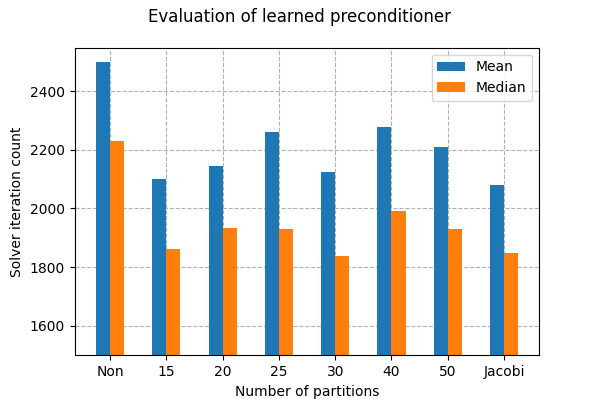
\includegraphics[width=1\textwidth]{plots/more_num_par_test_measure.png}
        \caption{Mean and median solver iteration count indicated by the colour of the bar from the evaluation of the learned preconditioners with different number of partitions indicated by the label.\\\\}
        \label{fig: more par test measure}
    \end{minipage}
    \begin{minipage}{.02\textwidth}
        
    \end{minipage}
    \begin{minipage}{.49\textwidth}
        \center
        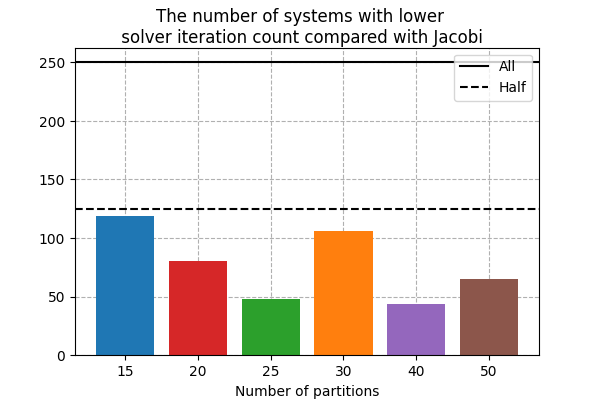
\includegraphics[width=1\textwidth]{plots/more_num_par_BvJ.png}
        \caption{Individual linear system comparison between the learned preconditioners with different number of partitions and Jacobi preconditioners with bar size corresponding to the number of systems where the learned preconditioner has a lower solver iteration count.}
        \label{fig: more par BvJ}
    \end{minipage}
\end{figure}


The second thing is that allowing accepting of worse state makes the learning worse for higher partition counts, as a consequence of the slower learning. It can most notably be seen for the 40 partition count run, purple learning curve. At learn step 324, the mean solver iteration count increases from 2238.3 to 2424.8, and then it does not get below the increase before it the number of learning steps maxed out. Compare this with the run with 25 partitions, which has increase in solver iteration count at learn iteration 215 and does get back to the iteration from before the increase at learn iteration 337. This problem could be improved with a smaller probability for accepting worse states, but then the learning might get stuck in a minimum. 

From the evaluations of the learned Preconditioners, figure \ref{fig: more par test measure} and \ref{fig: more par BvJ}, it is clear that using more partitions does not make the preconditioner better. Even with the change to the algorithm such that it returns the best found preconditioner during learning, as both the mean and median solver iteration count are on par, 15 and 30 partition, or worse than using the Jacobi preconditioning. And for all preconditioners the number of systems that have a lower solver iteration count compared to Jacobi is less than half.

\subsubsection{Fewer}
Because using more partitions did not improvement the learned preconditioners, we will now test with a smaller number of partitions. The partition count we will use in this test is \(\{1,2,3,4,5\}\) and that is the only difference between the runs. With the 200 base learning iterations to make the results comparable with the previous test with more partitions.


\begin{figure}[H]
    \begin{minipage}{.49\textwidth}
        \center
        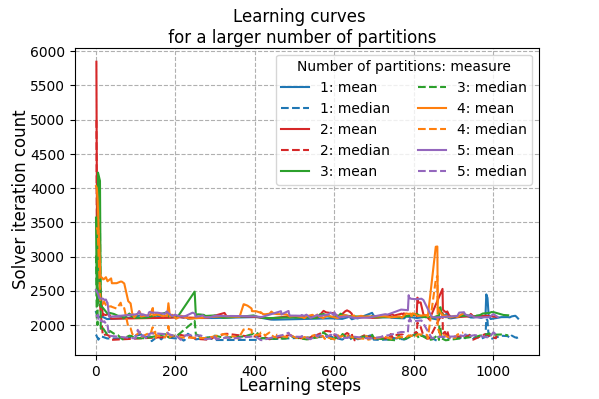
\includegraphics[width=1\textwidth]{plots/fewer_num_par_learning_curve.png}
        \caption{Learning curves for the testing with fewer number of partition, with the same structure as figure \ref{fig: more par learning curves}.\\}
        \label{fig: fewer par learning curves}
    \end{minipage}
    \begin{minipage}{.02\textwidth}
        
    \end{minipage}
    \begin{minipage}{.49\textwidth}
        \center
        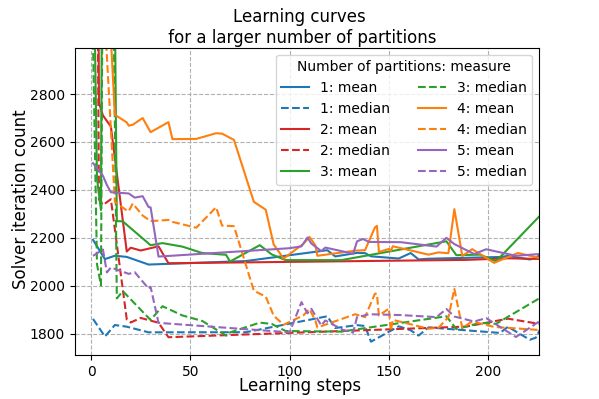
\includegraphics[width=1\textwidth]{plots/fewer_num_par_learning_curve_zoom.png}
        \caption{Learning curves for the test with fewer number of partition, the same data as figure \ref{fig: fewer par learning curves}, but zoomed in to the lower left corner to see the initial learning.}
        \label{fig: fewer par learning curves zoom}
    \end{minipage}
\end{figure}

The learning curves, seen in figures \ref{fig: fewer par learning curves} and \ref{fig: fewer par learning curves zoom}, are as excepted with fewer partitions has faster learning and it plateaus almost immediately. With the slowest run being with 4 partitions, orange learning curve, plateauing at the 100th learning step. The problem where accepting a worse state and not being able to get back to a similar solver iteration counts does not happen for these runs, as can be seen a bit after the 800th learning step, there is a major spike in solver iteration counts but all tests get back to previous iteration counts at around iteration 900. 

In the evaluation of the learned preconditioners, figure \ref{fig: fewer par test measure} and \ref{fig: fewer par BvJ}, we can see that they are all on par or slightly better than Jacobi preconditioning for all three measure. With using 1 partition begin best in this seed.


\begin{figure}[H]
    \begin{minipage}{.49\textwidth}
        \center
        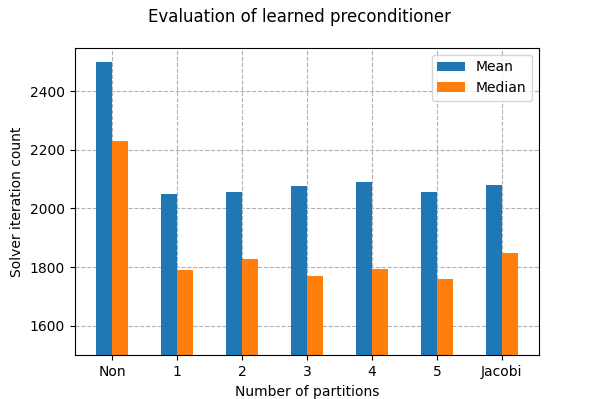
\includegraphics[width=1\textwidth]{plots/fewer_num_par_test_measure.png}
        \caption{Mean and median solver iteration count from the evaluate of the 5 learned preconditioners. The plot has the same structure as figure \ref{fig: more par test measure}.\\}
        \label{fig: fewer par test measure}
    \end{minipage}
    \begin{minipage}{.02\textwidth}
        
    \end{minipage}
    \begin{minipage}{.49\textwidth}
        \center
        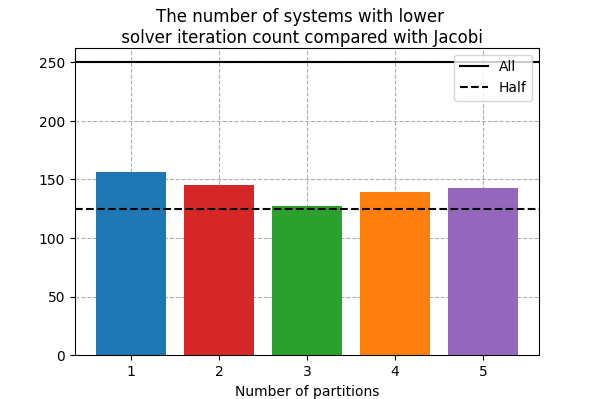
\includegraphics[width=1\textwidth]{plots/fewer_num_par_BvJ.png}
        \caption{Individual linear system comparison between the learned preconditioners and the Jacobi preconditioner. The plot has the same structure as figure \ref{fig: more par BvJ}.}
        \label{fig: fewer par BvJ}
    \end{minipage}
\end{figure}

The coefficients of the learned preconditioners with fewer number partitions, table \ref{tabel: fewer par coefficients}, are not equal, because of the inheritant randomness of the algorithm, but the values are close with an average value of \(-0.013641246\) and standard deviation of \(0.00445245\). Because of this and the increased speed in learning. The new standard preconditioner will have 1 partition in the superdiagonal.


\begin{table}[H]
    \center
    \begin{tabular}{|r|l|}
        \hline
        Par & Partition coefficients \\ \hline
        1 &\([-0.01463557]\) \\
        2 &\([-0.01678746, -0.02122048]\) \\
        3 &\([-0.00676193, -0.01237617, -0.01208201]\) \\
        4 &\([-0.02033992, -0.01883074, -0.01200618, -0.01339265]\)\\
        5 &\([-0.01600863, -0.00575484, -0.00860635, -0.01501886, -0.0107969]\) \\ \hline
    \end{tabular}
    \caption{Table of the learned preconditioners coefficients, with a row for each different number of partitions.}
    \label{tabel: fewer par coefficients}
\end{table}

From both of the test with changing the number of partitions we did not solve the problem of the preconditioner plateauing, as was the intention with the tests, but we did confirm that using more partitions would result in slower learning, to the point of a good preconditioner being unlearnable, and with fewer learning faster and plateauing quickly. 

\subsection{Number of diagonals}\label{sec: num super}
The next change to the structure we will test is the is the number of superdiagonals with coefficients. The initial reason for using only the first superdiagonal was to keep the preconditioner as spares as possible, to decreases the computational cost of the matrix vector product for the preconditioner. For these runs we will test with \(\left\lbrace 1,2,3,4,5\right\rbrace\) super diagonals with one partition in each, as to keep the number of coefficients low for faster learning. 

\begin{figure}[H]
    \center
    \begin{minipage}{.49\textwidth}
        \center
        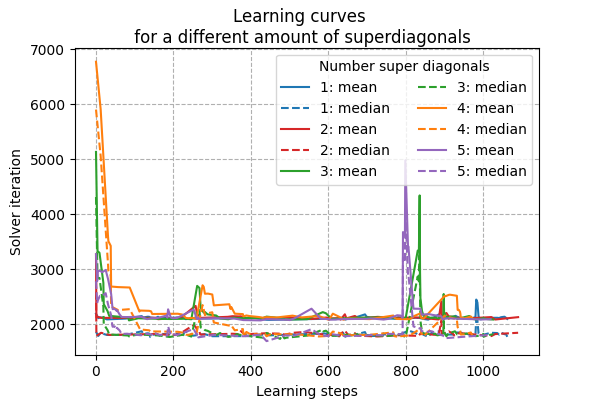
\includegraphics[width=1\textwidth]{plots/num_super_learn_curve.png}
        \caption{Learning curves for different number of superdiagonals in the preconditioner, with line style indicating mean or median solver iteration counts.\\}
        \label{fig: num super par learning curves}
    \end{minipage}    
    \begin{minipage}{.02\textwidth}
        
    \end{minipage}
    \begin{minipage}{.49\textwidth}
        \center
        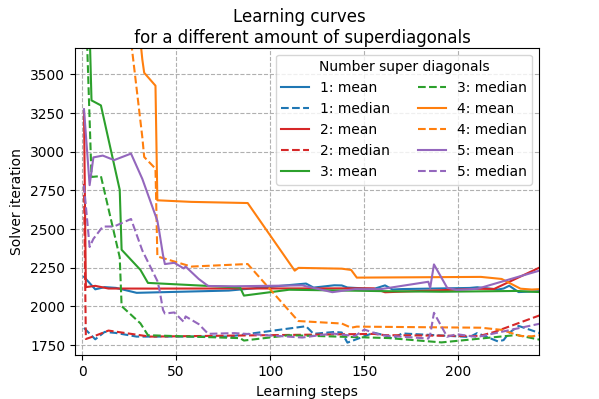
\includegraphics[width=1\textwidth]{plots/num_super_learn_curve_zoom.png}
        \caption{Learning curves for different number of super diagonals in the preconditioner, same data as figure \ref{fig: num super par learning curves} but zoomed in to the lower left corner to see the initial learning steps.}
        \label{fig: num super par learning curves zoom}
    \end{minipage}
\end{figure}

\begin{figure}[H]
    \center
    \begin{minipage}{.49\textwidth}
        \center
        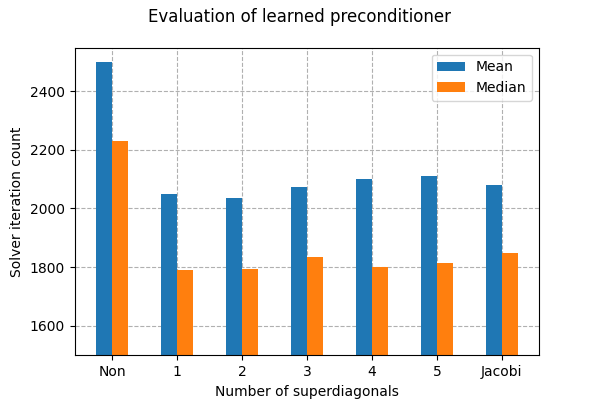
\includegraphics[width=1\textwidth]{plots/num_super_test_measure.png}
        \caption{Mean and median solver iteration count from the evaluation of the learned preconditioners with different number of super diagonals, with unpreconditioned and Jacobi preconditioned solver iteration count added for Comparison.}
        \label{fig: num super par test measure}
    \end{minipage}
    \begin{minipage}{.02\textwidth}
        
    \end{minipage}
    \begin{minipage}{.49\textwidth}
        \center
        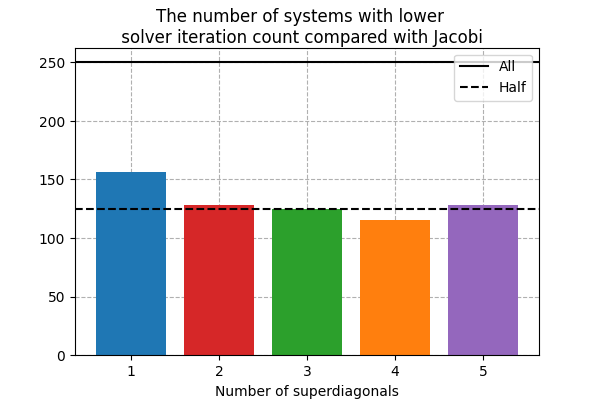
\includegraphics[width=1\textwidth]{plots/num_super_BvJ.png}
        \caption{Bar graph showing how many individual preconditioned systems have a lower solver iteration count compared to Jacobi preconditioning.\\\\}
        \label{fig: num super par BvJ}
    \end{minipage}
\end{figure}

From the learning curves, figure \ref{fig: num super par learning curves} and \ref{fig: num super par learning curves zoom}, we see similar results as the previous test, with regards to the speed of the learning and marginal differences in mean and median solver iteration counts. In the evaluation of the learned preconditioners it is as excepted with what was seen in the learning curves. Slight differences in the mean and median solver iteration counts increasing with more superdiagonals, figure \ref{fig: num super par test measure}. And in the individual iteration counts comparison, figure \ref{fig: num super par BvJ}, 1 super diagonal clearly preforms the best of the five test. Therefore we conclude that using 1 super diagonal, with no significant difference in evaluation, the faster learning, and most importantly the faster matrix vector product by having fewer nonzero entries.


% From the learning curves, figure \ref{fig: num super par learning curves} and \ref{fig: num super par learning curves zoom}, we see the similar results as the previous test, with regards to the speed of the learning, fewer coefficients leads to faster learning. There is also only a marginal differences in the learning data solver iteration counts with higher number of super diagonal being slightly worse. In the evaluation of the learned preconditioners on the testing data it is as excepted with what was seen in the learning curves. With similar conclusions, marginal differences in the mean and median solver iteration counts, figure \ref{fig: num super par test measure}, and in the individual iteration counts comparison, figure \ref{fig: num super par BvJ}, having a clear best using 1 super diagonal. Meaning it is easy conclude that using 1 super diagonal, with no significant difference in testing, the faster learning, and most importantly the faster matrix vector by the fact having fewer nonzero value.

\newpage
\subsection{Super- and subdiagonals}\label{sec: super sub}
Because using more superdiagonals did not improve the preconditioner, we will go in the other direction by using both the super- and subdiagonals. We will test using \(\left\lbrace 1,2,3,4\right\rbrace\) super- and subdiagonals with 1 partition in each diagonal, leading to \(\left\lbrace 2,4,6,8\right\rbrace\) different coefficients that needs to be learned. 

Immediately from the learning curves in figure \ref{fig: super sub learning curves} seed 0, we see a sizeable improvement. With the plateaued mean solver iteration count around 1750 and median around 1500, compared with the runs of previous section \ref{sec: num super} having plateaued around mean of 2100 and median of 1800 solver iteration count. Because of the large improvement, the test was run again with a different seed to ensure improvement was not because of the seed of the data set and start conditions of the preconditioners. In the learning curves of this second run we see that the learning curves plateaus at similar solver iteration counts. With the only anomaly being the run with 4 super and 4 subdiagonals, the grey curve. This happened because in implementation the coefficients of the preconditioner is first generated, it then tries to change one coefficients to see if an improvement occurred, but in the first learning iteration there is no point of comparison, meaning the preconditioner is accepted if all preconditioned systems converged and there is the problem. With bad starting coefficients there may not be a change that can be made to the coefficients such that all systems converge. Even with the bad start and the slower learning, because of the 8 coefficients that needs to be learned, its learning curve still gets almost as good results as the runs in this test and a better results compared test from the previous sections.


\begin{figure}[H]
    \center
    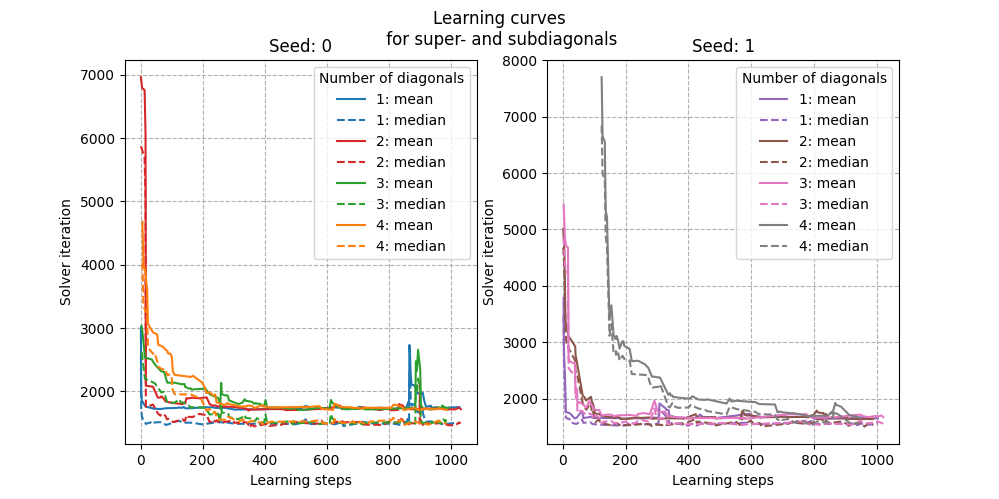
\includegraphics[width=1\textwidth]{plots/super_sub_learn_curve.png}
    \caption{Learning curves for the preconditioner that uses both the super and subdiagonal with a plot for each of the two seeds, with colour corresponding to a different number of super- and subdiagonals  and linestyle corresponding to mean or median solver iteration count.}
    \label{fig: super sub learning curves}
\end{figure}

In the evaluation of the learned preconditioners there also is a major improvement. The mean and median solve iteration counts is around 400 iterations fewer compared to Jacobi preconditioning for all diagonal counts and both seeds, figure \ref{fig: super sub test measure}. Where the previous preconditioners with only the superdiagonal was on par with jacobi preconditioning. In the individual comparison, figure \ref{fig: super sub BvJ}, there is a similar improvement, because all preconditioners have more than 240 systems with lower iteration count compared to Jacobi preconditioning, with 1 super- and 1 subdiagonal begin best for both seeds.

\begin{figure}[H]
    \center
    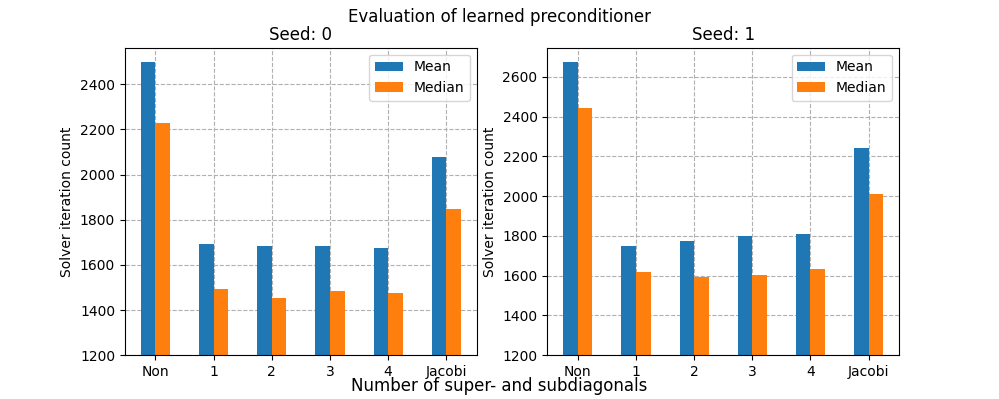
\includegraphics[width=1\textwidth]{plots/super_sub_test_measure.png}
    \caption{Mean and median solver iteration count for the evaluation of the learned preconditioners with different number of super- and subdiagonals, with a plot for each of the two seeds. With colour corresponding to mean or median solver iteration count.}
    \label{fig: super sub test measure}
\end{figure}

\begin{figure}[H]
    \center
    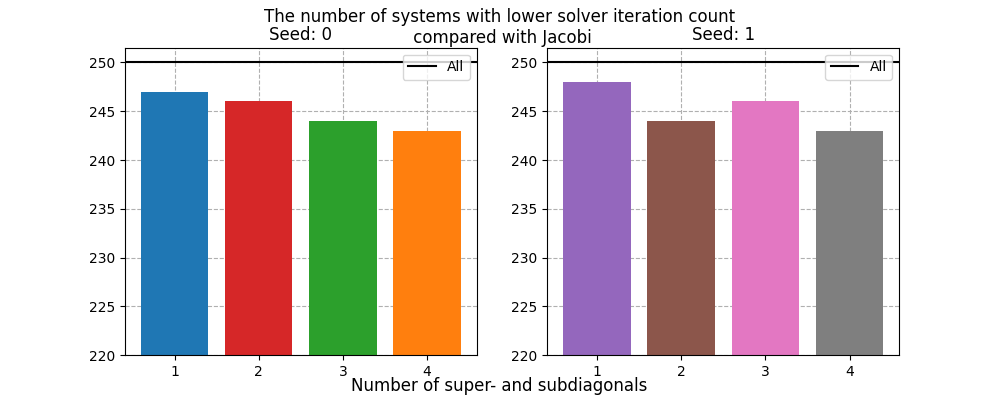
\includegraphics[width=1\textwidth]{plots/super_sub_BvJ.png}
    \caption{Bar graph showing how many individual systems that has a lower solver iteration count with the learned preconditioners compared with its Jacobi preconditioned counterpart, with a plot for each of the two seeds.}
    \label{fig: super sub BvJ}
\end{figure}


\subsubsection{Number of partitions}
Because of the significant change made to the preconditioner, we will test if the number of partitions now will have any effect on the learned preconditioners. The number of partitions will be symmetric for the super- and subdiagonal and the number of partitions in the test will be \(\left\lbrace 1,2,3,4\right\rbrace\).

% Now that we have a preconditioner with changed structure we wil do the runs with change in partition count with one super and sub diagonal, to see if it now will improve the preconditioner or that the results will be similar to the previous testing of the type.
From the learning curves, figure \ref{fig: par super sub learning curves}, we see similar results as the previous test with different number of partitions in section \ref{sec: num par}. That is more partitions decrease the learning rate with marginal differences in outcome. With one partition count is better in one measure but worse in another. For example with 1 partition has the highest number of individual systems that has a lower solver iteration count compared to Jacobi preconditioned systems, figure \ref{fig: par super sub BvJ}, but has a worse mean and median solver iteration count compared to the learned preconditioner with 2 partitions. 

\begin{figure}[H]
    \center
    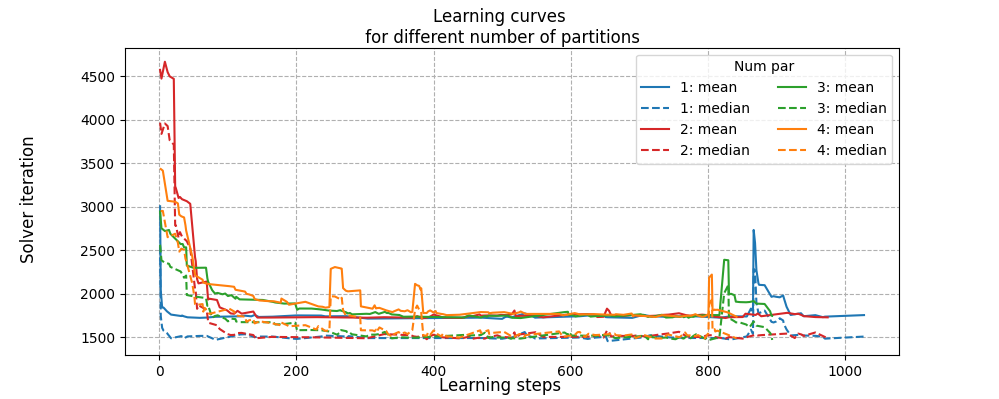
\includegraphics[width=1\textwidth]{plots/par_super_sub_learn_curve.png}
    \caption{Learning curves for learning preconditioners with 1 super- and subdiagonal. With colour corresponding to a different number of partitions and linestyle the mean or median solver iteration count.}
    \label{fig: par super sub learning curves}
\end{figure}


\begin{figure}[H]
    \center
    \begin{minipage}{.49\textwidth}
        \center
        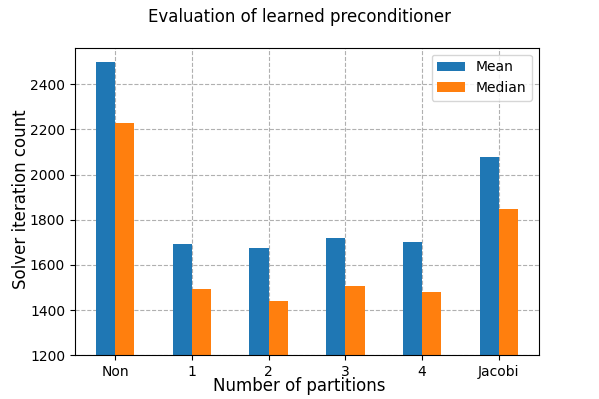
\includegraphics[width=1\textwidth]{plots/par_super_sub_test_measure.png}
        \caption{Mean (blue) and median (orange) solver iteration counts from the evaluation of the learned preconditioners, with unpreconditioned and Jacobi preconditioning for comparison.\\}
        \label{fig: par super sub test measure}
    \end{minipage}
    \begin{minipage}{.02\textwidth}
        
    \end{minipage}
    \begin{minipage}{.49\textwidth}
        \center
        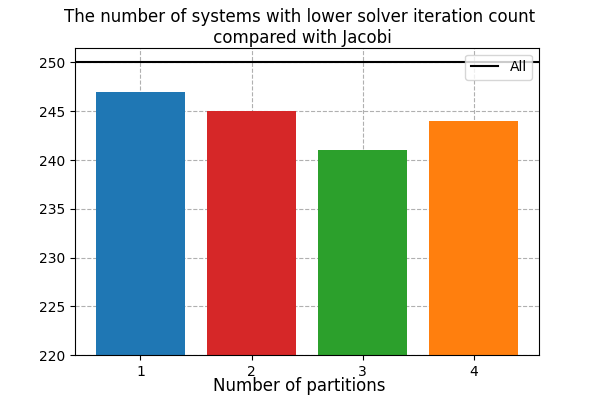
\includegraphics[width=1\textwidth]{plots/par_super_sub_BvJ.png}
        \caption{Bar Graph showing how many individual systems that has a lower solver iteration count with the learned preconditioners compared with its Jacobi preconditioned counterpart., With an y-axis offset of 220.}
        \label{fig: par super sub BvJ}
    \end{minipage}
\end{figure}


\begin{table}[H]
    \center        
    \begin{tabular}{|r|ll|}
        \hline
        Par & Superdiagonal & Subdiagonal \\ \hline
        1 & \([-0.059248]\) & \([-0.054830]\) \\
        2 & \([-0.063006, -0.064121]\) & \([-0.059046, -0.056173]\) \\ 
        3 & \([-0.064320, -0.065399, -0.058531]\) & \([-0.055929, -0.074727, -0.055672]\) \\
        4 & \([-0.046214, -0.058072, -0.047579, -0.063756]\) & \([-0.044746, -0.060495, -0.049910, -0.067014]\) \\\hline
    \end{tabular}
    \caption{Table of the learned preconditioners coefficients, with a row for each different number of partitions, columns for the superdiagonal coefficients and one for the subdiagonal coefficients.}
    \label{table: par super sub coefficients}
\end{table}

For the coefficients of the learned preconditioners, we again see similarities to section \ref{sec: num par}, that being the coefficients are similar, even between the super- and subdiagonal, table \ref{table: par super sub coefficients}. Because of this, with only slight differences in learning outcome and the faster learning we can again conclude that using 1 partition each diagonal gets better learned preconditioners.

\subsubsection{Symmetry}
Because of the similarities of the coefficients between the super- and subdiagonal. We will repeat the test from section \ref{sec: super sub} but with symmetric preconditioners, as this would half the number of coefficients that needs to be learned and therefore faster learning.

\begin{figure}[H]
    \center
    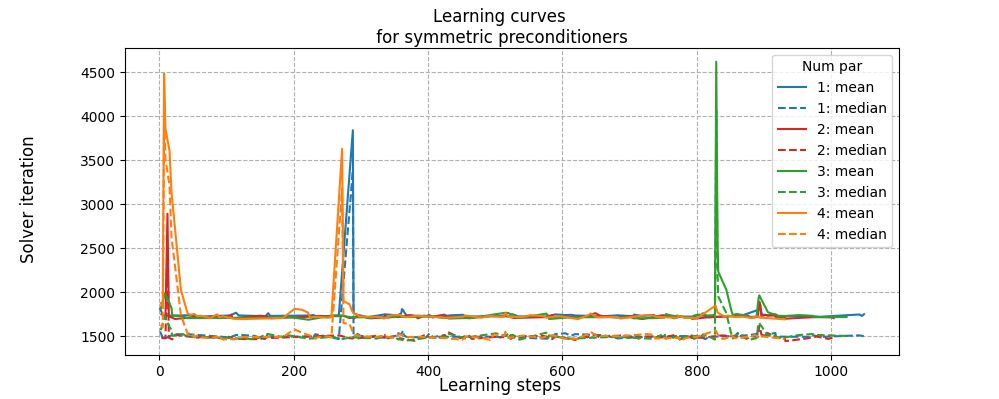
\includegraphics[width=\textwidth]{plots/sym_super_sub_learn_curve.png}
    \caption{Learning curves for from the learning of symmetric preconditioners with 1 super- and subdiagonal. WIth colour corresponding to a different number of partitions and linestyle to mean or median solver iteration count.}
    \label{fig: sym super sub learning curves}
\end{figure}

On major difference in the learning for all of the runs is the actual 
+run time of each of the configurations. When compared with the similar test of section \ref{sec: super sub} it has increased significantly. The cause of the increase in run time is that changes made to the preconditioners during learning increased the solver iteration counts significantly of most of the systems and therefore some of the learning steps takes significantly longer than other. An example can be seen as the spikes in figure \ref{fig: sym super sub learning curves} where such a state was accept. The cause of large increase in solver iteration count because the change made to a coefficient has a larger affect on the preconditioners. A solution would entail a change in the distribution generating the changes made to the coefficients, but changes to this distribution would also have effects on the learning time. With this being the only major difference in the learning of the preconditioner.

In the evaluation of the learned preconditioners, figure \ref{fig: sym super sub test measure} and \ref{fig: sym super sub BvJ}, there is only marginal differences between the solver iteration counts of these tests and the test with unsymmetric preconditioners in section \ref{sec: super sub} seed 0. Because of the increase in run time of the learning algorithm we conclude that using a the symmetric variant of out preconditioner bad.

\begin{figure}[H]
    \center
    \begin{minipage}{.49\textwidth}
        \center
        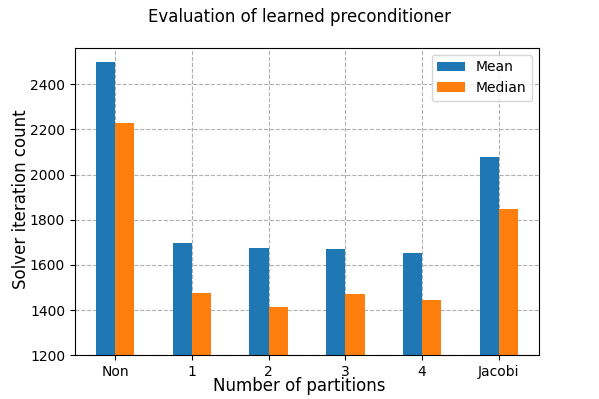
\includegraphics[width=1\textwidth]{plots/sym_super_sub_test_measure.png}
        \caption{Mean (blue) and median (orange) solver iteration counts from the evaluation of the learned preconditioners, with unpreconditioned and Jacobi preconditioning for comparison.}
        \label{fig: sym super sub test measure}
    \end{minipage}
    \begin{minipage}{.02\textwidth}
        
    \end{minipage}
    \begin{minipage}{.49\textwidth}
        \center
        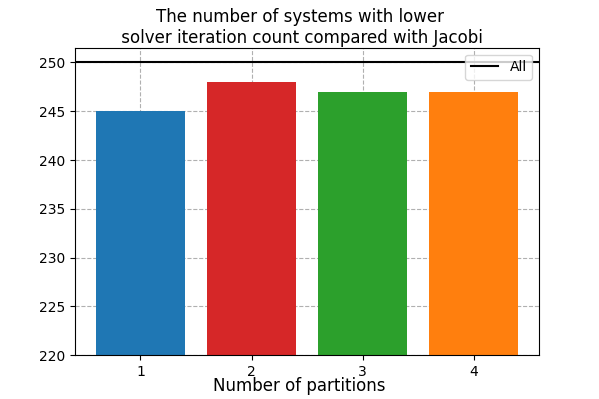
\includegraphics[width=1\textwidth]{plots/sym_super_sub_BvJ.png}
        \caption{Bar graph showing how many individual systems that has a lower solver iteration count with the learned preconditioners compared with its Jacobi preconditioned counterpart.}
        \label{fig: sym super sub BvJ}
    \end{minipage}
\end{figure}




\subsection{Testing the algorithm on larger systems}
With the learning algorithm and structure of the preconditioner gotten to a point where it can reliably learn a preconditioner than can improve the mean solver iteration count by 2000 iterations compared to a trivial preconditioner. There is one parameter that have not changed and that is the size of the 2-dimensional discrete laplace operator used in the training and test data sets. Because no testing has been done on different size laplace operators, importantly larger sizes. The conclusions made from the different tests, especially on the parameter choice and the structure of preconditioner, might be specialized towards the current system size and perturbations. One change that as made to the structure of the preconditioner that is specialized was made in section \ref{sec: jacobi shift}. That is the change from an identity diagonal to the Jacobi preconditioner as the diagonal. Because if the matrices in our data sets had diagonals closer to an identity diagonal, Jacobi preconditioning would not make any difference or if the diagonals were close to zero Jacobi preconditioner would have and adverse effect on the preconditioner, and it could therefore struggle to learn a good preconditioner. 

Therefore the next test we will change the size of the systems sizes and the perturbations applied to them. Unfortunately this is not as simple as it would seem, because of the condition in our learning algorithm that all systems must converge for a change made to the preconditioner to be accepted. This condition was original implemented because of the problem of comparison between learning iterations where different system does not converge, as it could skew with results of the comparisons in either direction. 

To find a suitable larger size and larger perturbations, preliminary testing different size and perturbation distribution data sets on the linear solvers. In these preliminary tests there were almost always at least one or two systems that did not converge. We conclude that it is because of the perturbation distribution being the normal distribution. By having a larger variance and larger system sizes there is more perturbations that is needed to be generated and therefore more likely generate an outlier, that would make the final matrix ill-conditioned. To get more control of outliers we change the distribution that generate the perturbations to a uniform distribution with mean of 1 and variable range, \(Uni(1-r,1+r)\). Testing with this distribution we landed on the 1-dimensional discrete laplacian operator size of 65 resulting in a final system size of 4225 and a range of 0.45 for the perturbations. With these data generation parameters we ran the learning algorithm with 50 base learning steps on 4 different seeds and preconditioner having 1 super- and 1 subdiagonal with 1 partition each. 

\begin{tabular}{l} \\ \end{tabular}

\begin{table}[H]
    \center
    \begin{tabular}{|l|l|r||l|l||l|r|r|}
        \hline
        \(N\) & \begin{tabular}{@{}l@{}} Pertubation \\ distribution \end{tabular}  & Amount &\begin{tabular}{@{}l@{}}Base learning \\ steps \end{tabular}& Learn Scales &\begin{tabular}{@{}l@{}}Initial coefficient \\distribution \end{tabular}  &\begin{tabular}{@{}l@{}}Number of \\ partitions \end{tabular} & Diagonals\\\hline
        65 & \(Uni(0.55,1.45)\) & 250 & 50 & \(\pm\{1,0.5,0.25\}\) & \(N(0,0.05^2)\) & 1 & \((1,-1)\)\\ \hline
    \end{tabular}
    \caption{Table of the run parameter configuration where the columns corresponds to in order: the size of the 1-dimension discrete laplace operator; the initial perturbations on the data; the amount of systems in the data sets; the base number of learning iterations; the scales of the exploration changes; the distribution of the initial coefficients; the number of partitions; the diagonals used.}
    \label{table: large test config}
\end{table}

\begin{figure}[H]
    \center
    \begin{minipage}{.49\textwidth}
        \center
        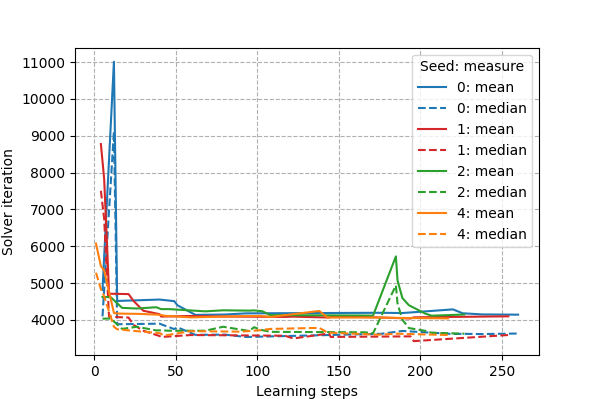
\includegraphics[width=1\textwidth]{plots/large_learning_curve_zoom.png}
        \caption{Learning curves for from the learning of the larger systems, where the colour of the curve corresponds to the different seeds.\\\\}
        \label{fig: large learning curves}
    \end{minipage}
    \begin{minipage}{.02\textwidth}
        
    \end{minipage}
    \begin{minipage}{.49\textwidth}
        \center
        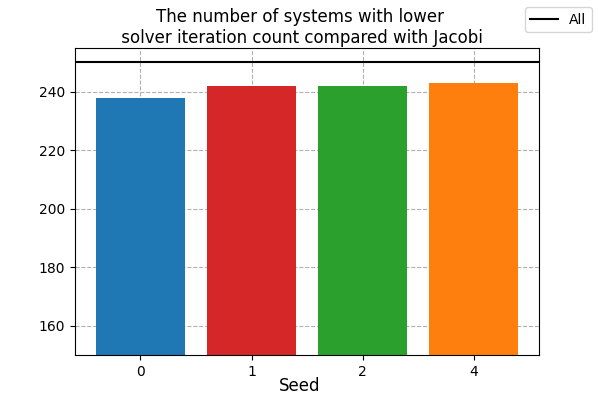
\includegraphics[width=1\textwidth]{plots/large_BvJ.png}
        \caption{Graph showing how many individual systems that has a lower solver iteration count with the learned preconditioners compared with its Jacobi preconditioned counterpart from the different seeds. With an y-axis offset of 150.}
        \label{fig: large BvJ}
    \end{minipage}
\end{figure}

\begin{figure}[H]
    \center
    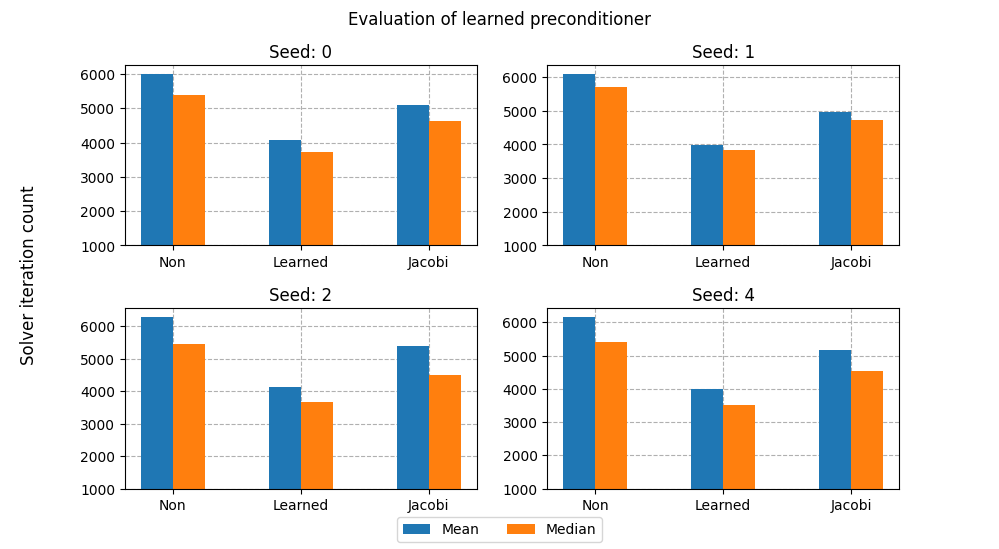
\includegraphics[width=0.9\textwidth]{plots/large_test_measure.png}
    \caption{Mean (blue) and median (orange) solver iteration counts from the evaluation of the learned preconditioners, with unpreconditioned and Jacobi preconditioning for comparison, with a plot for each of the seeds.}
    \label{fig: large test measure}
\end{figure}
    

From learning curves in figure \ref{fig: large learning curves} we can see what we have seen many times in the previous tests. That is the mean and median solve iteration counts decrease during the learning quickly and therefore plateaus. For example for seed 1, red curve, starts with a mean solver iteration count 8773.2 and decreases to a count a bit above 4000, and similar curves for the other seeds.

In the evaluation of the learned preconditioners, we can see that the preconditioners decreases the mean and median solver iteration count by approximately 2000 iterations compared to using no preconditioner and 1000 compared with Jacobi preconditioning, figure \ref{fig: large test measure}. For the individual comparisons in figure \ref{fig: large BvJ} that around 240 system with the learned preconditioner have a lower solver iteration count compared with using Jacobi preconditioning. Meaning it is fair to say that the algorithm has learned a good preconditioner for the larger system sizes for all four seeds.


